% circuit-sim-lab-report — report.tex
% Course 0714-EEE-2102, Circuit Simulation Laboratory
% Experiment 7 — input and output characteristics of a BJT in CB, CE and CC
%
% Compile (twice, from Lab_report_latex/):
%   env pdflatex -interaction=nonstopmode report.tex

\documentclass[12pt,a4paper]{article}

% ----- Page geometry: A4, 1 inch margins all sides -----
\usepackage[margin=1in]{geometry}

% ----- Times New Roman (text + math) -----
\usepackage{newtxtext,newtxmath}

% ----- Spacing: 1.5 line spacing, 6 pt paragraph spacing -----
\usepackage{setspace}
\onehalfspacing
\usepackage{parskip}          % paragraph gaps instead of indents
\setlength{\parskip}{6pt plus 1pt}

% ----- Math, SI units -----
\usepackage{amsmath}
\usepackage{siunitx}

% ----- Graphics, tables, captions, floats -----
\usepackage{graphicx}
\usepackage{booktabs}
\usepackage{caption}
\usepackage{float}
\usepackage{array}
\usepackage{needspace}
\graphicspath{{../graphs/}{../schematics/}{./figures/}}

% ----- Lists: compact, guide-style itemization -----
\usepackage{enumitem}
\setlist{nosep, leftmargin=2em, label=\textbullet}

% ----- Front matter and PDF output -----
\usepackage{pdfpages}
\usepackage[hidelinks]{hyperref}

% ----- Headings: bold, left-aligned, 14/15 pt -----
\usepackage{titlesec}
\titleformat{\section}
{\normalfont\Large\bfseries}{\thesection}{0.8em}{}
\titleformat{\subsection}
{\normalfont\large\bfseries}{\thesubsection}{0.8em}{}
\titlespacing*{\section}{0pt}{*3}{*2}
\titlespacing*{\subsection}{0pt}{*2.5}{*1.5}

% ----- Captions: centered, 11 pt, figures below / tables above -----
\captionsetup{font=small, labelfont=normalfont, justification=centering}
\captionsetup[table]{position=above, skip=4pt}
\captionsetup[figure]{position=below, skip=4pt}
\newcommand{\schematicpanel}[2]{%
	\begin{minipage}[t]{0.48\textwidth}\centering
		\includegraphics[width=\linewidth]{#2}
		\\[2pt]\textbf{(#1)}
\end{minipage}}

% ----- Page number: bottom-center -----
\usepackage{fancyhdr}
\pagestyle{fancy}
\fancyhf{}
\fancyfoot[C]{\thepage}
\renewcommand{\headrulewidth}{0pt}

% ----- Experiment number: sections then number 7.1-7.10 -----
\newcommand{\expnumber}{7}
\renewcommand{\thesection}{\expnumber.\arabic{section}}

\begin{document}
	
	% =====================================================================
	% FRONT MATTER (pages 1-2): cover page and task sheet
	% =====================================================================
	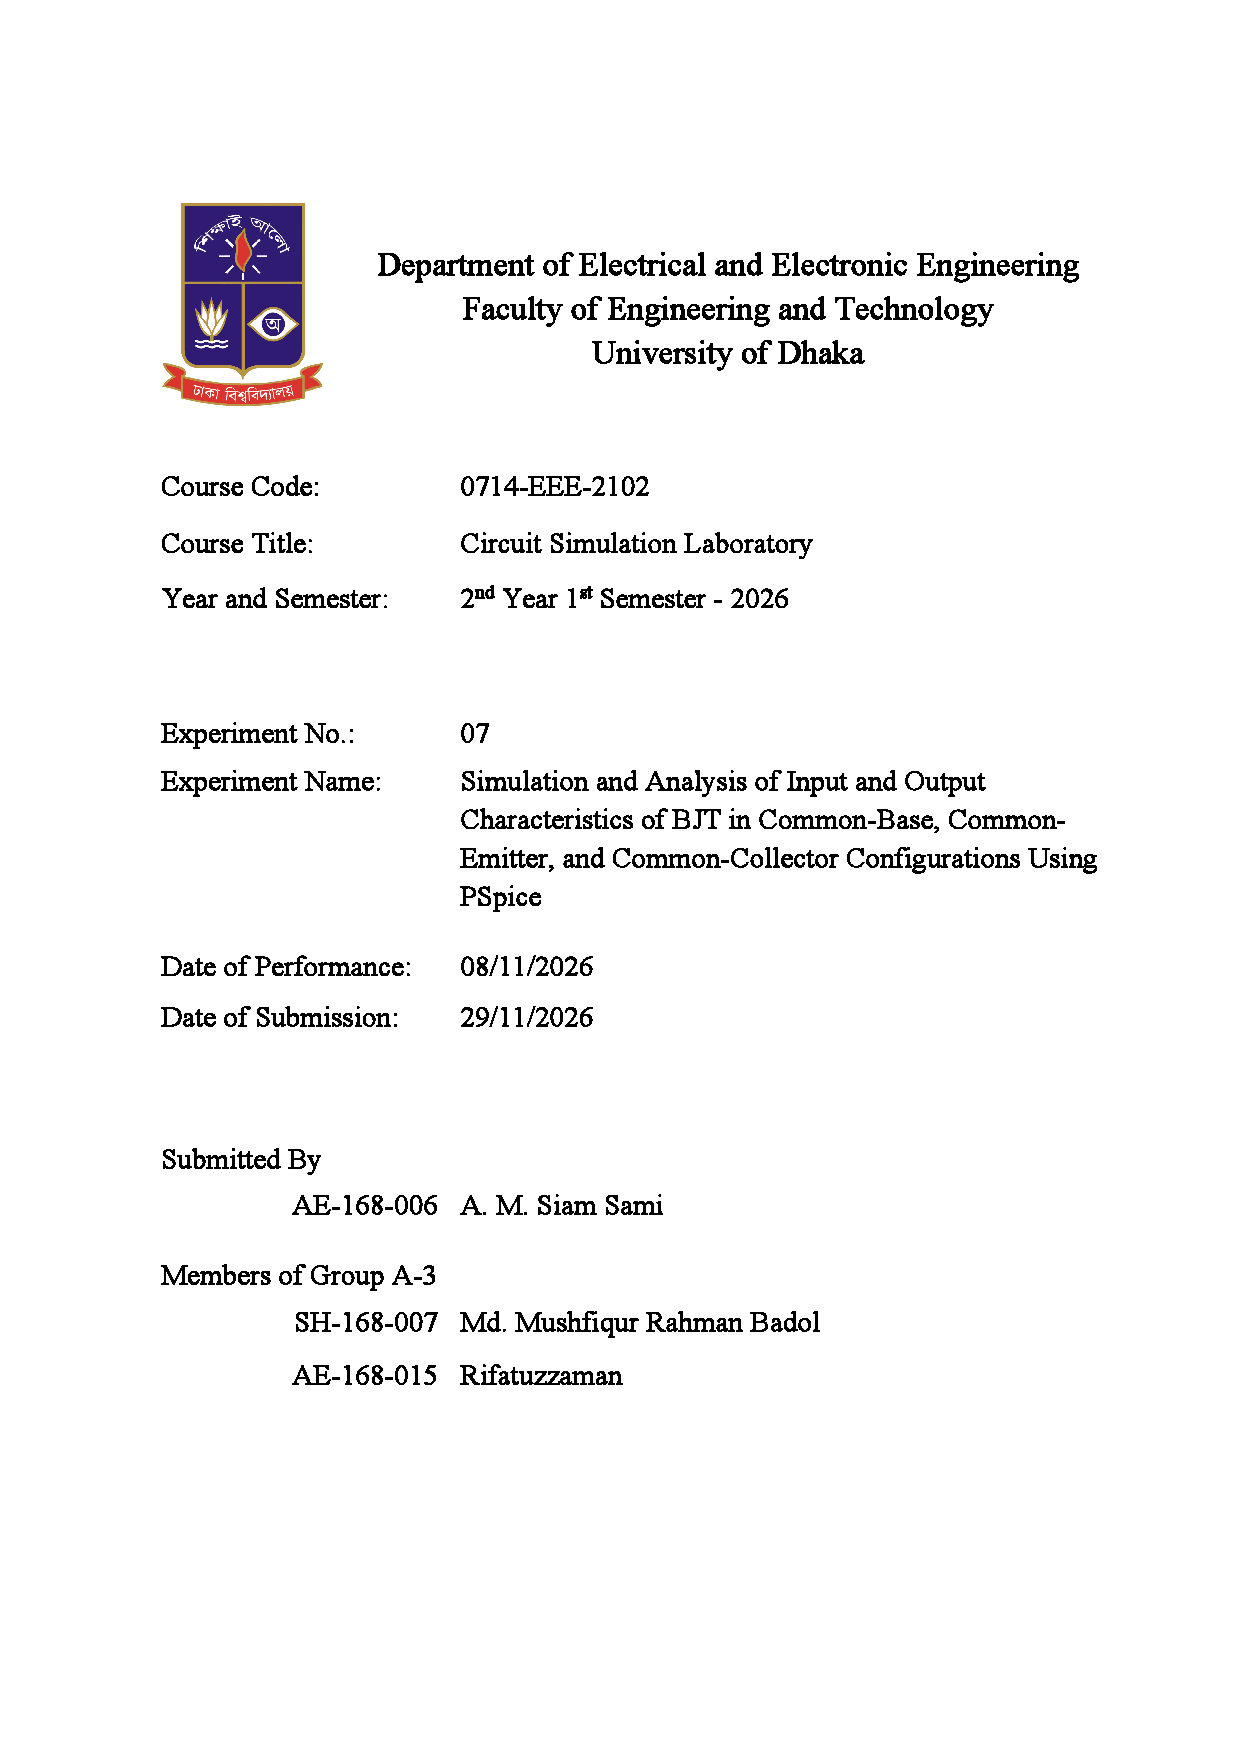
\includepdf[pages={1,2,3}]{../covers.pdf}
	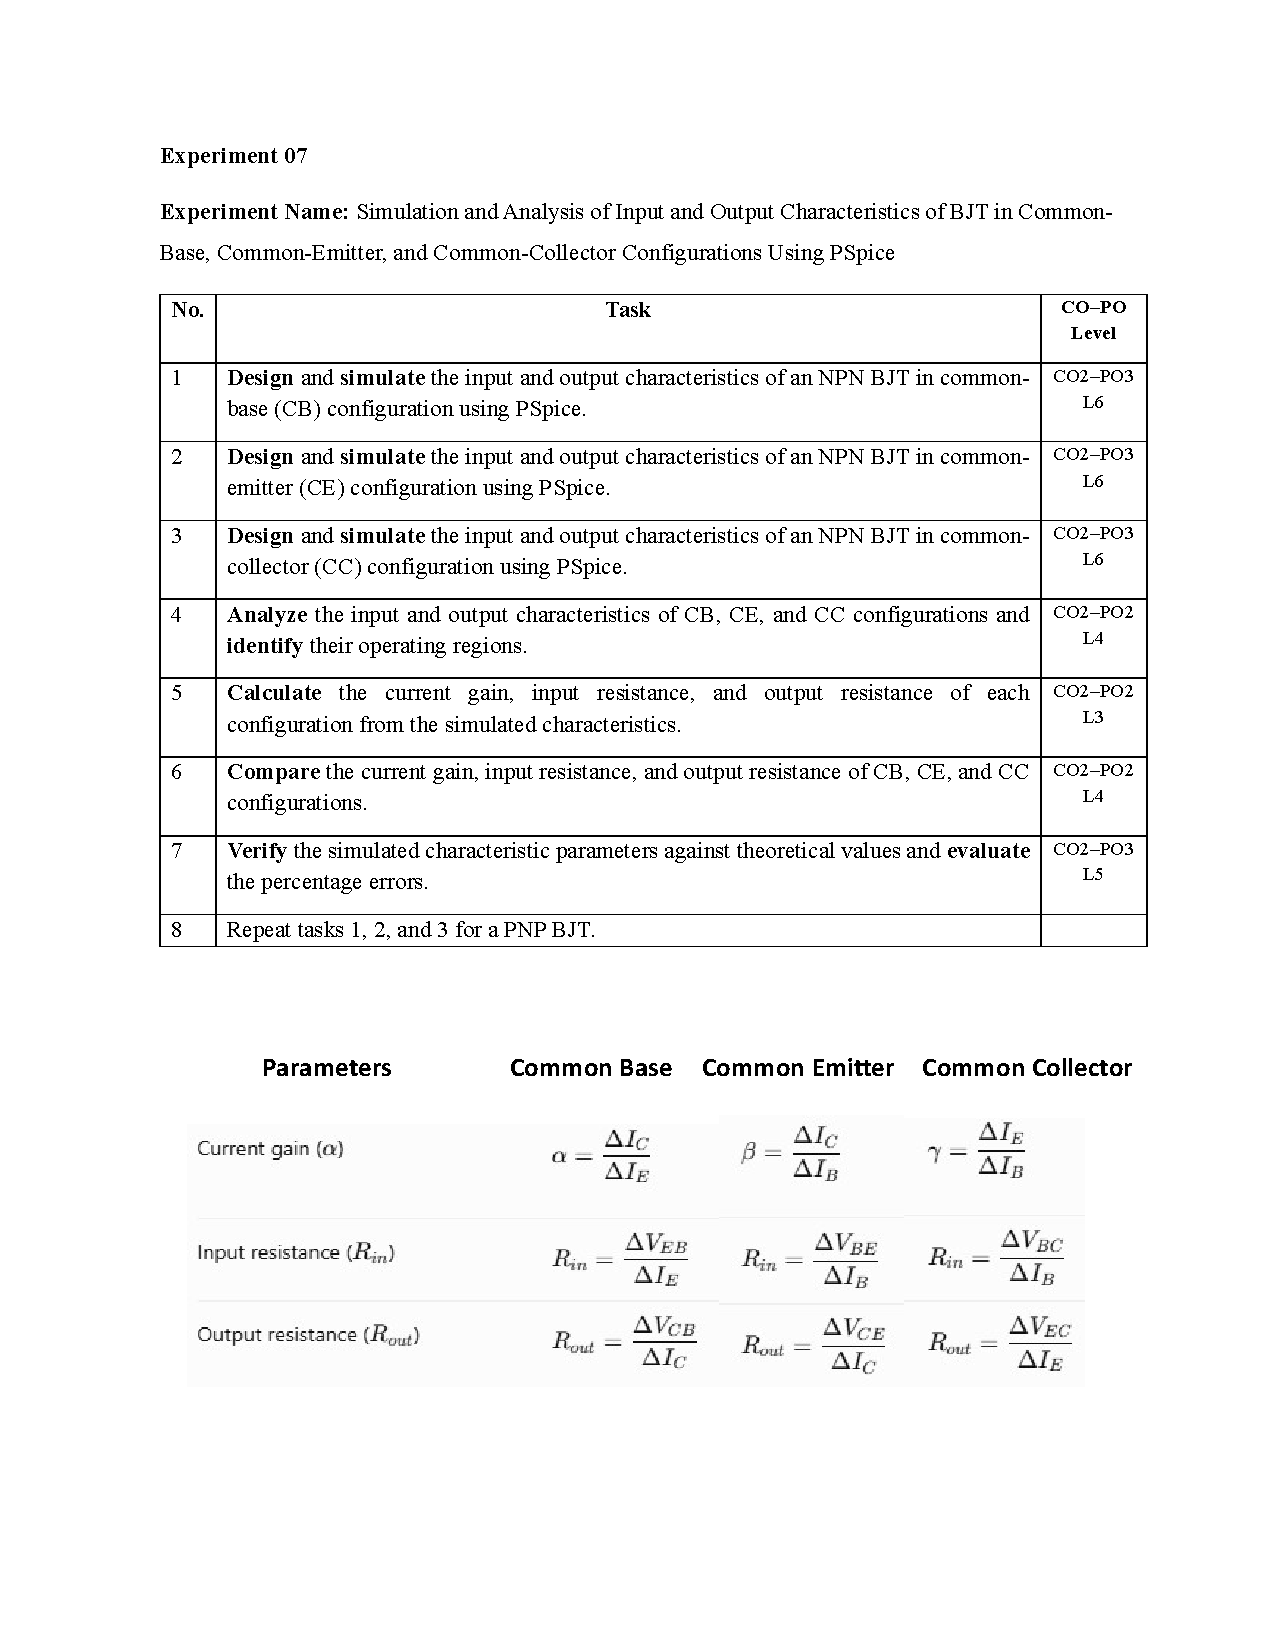
\includepdf[pages={1}]{../Exp 07.pdf}
	\setcounter{page}{1}
	
	% =====================================================================
	% HEADER BLOCK
	% =====================================================================
	\begin{center}
		{\large\bfseries Experiment No. \expnumber}\\[4pt]
		{\large\bfseries Name of the Experiment: Simulation and Analysis of
			Input and Output Characteristics of BJT in Common-Base,
			Common-Emitter, and Common-Collector Configurations Using PSpice}
	\end{center}
	\vspace{6pt}
	
	% =====================================================================
	\section{Objective}
	% =====================================================================
	The purposes of this experiment are-
	\begin{enumerate}[label=\roman*.]
		\item To design and simulate the input and output characteristics of an NPN BJT (2N3904) in the common-base, common-emitter and common-collector configurations using PSpice.
		\item To repeat the characteristic families for a PNP BJT (2N3906) with all supply voltages and currents reversed.
		\item To identify the cutoff, active and saturation regions of each configuration from the simulated curves.
		\item To determine the current gain, input resistance and output resistance of every configuration from the simulated characteristics and to verify them against the theoretical values through percentage-error analysis.
	\end{enumerate}
	
	% =====================================================================
	\section{Theory}\label{sec:theory}
	% =====================================================================
	A bipolar junction transistor consists of two pn junctions that share a
	thin base region \cite{ref:sedra}. In the NPN device the emitter and collector are n-type
	and the base is p-type; in the PNP device the doping is reversed. In the
	forward-active region the emitter-base junction is forward biased and the
	collector-base junction is reverse biased. Nearly all the carriers
	injected by the emitter are collected by the collector, so the collector
	current is a fraction $\alpha$ of the emitter current and the base
	current is the small remainder. The three terminal currents are related
	by Kirchhoff's current law as
	\begin{equation}
		I_E = I_C + I_B .
		\label{eq:kcl}
	\end{equation}
	For the PNP device the currents flow in the opposite sense, entering the
	emitter and leaving through the collector and the base. All the
	characteristics of the PNP transistor are therefore the mirror images of
	the NPN curves, and they are plotted in this report as magnitudes so
	that the two devices can be compared directly.
	
	Which terminal is held common to the input and the output decides the
	configuration and, with it, which quantity is the input and which is the
	output. In the common-base (CB) connection the base is grounded, the
	input is applied between emitter and base and the output is taken
	between collector and base. In the common-emitter (CE) connection the
	emitter is grounded, the input is between base and emitter and the
	output between collector and emitter. In the common-collector (CC)
	connection the collector is grounded, the input is again between base
	and emitter, and the output is taken at the emitter \cite{ref:theraja}.
	The same device
	therefore presents three different pairs of characteristics, because
	each connection measures the transistor from a different pair of
	terminals.
	
	Each configuration has an input characteristic, in which the input
	current is plotted against the input voltage at a fixed output voltage,
	and an output characteristic, in which the output current is plotted
	against the output voltage for a set of fixed input currents. The task
	sheet defines the three current gains from increments of the output
	characteristics taken at a constant output voltage,
	\begin{equation}
		\alpha = \left.\frac{\Delta I_C}{\Delta I_E}\right|_{V_{CB}}, \qquad
		\beta = \left.\frac{\Delta I_C}{\Delta I_B}\right|_{V_{CE}}, \qquad
		\gamma = \left.\frac{\Delta I_E}{\Delta I_B}\right|_{V_{CE}},
		\label{eq:gains}
	\end{equation}
	for the CB, CE and CC connections respectively. Equation~\eqref{eq:kcl}
	holds for increments as well, $\Delta I_E = \Delta I_C + \Delta I_B$, so
	that only two of the three gains are independent,
	\begin{equation}
		\gamma = 1 + \beta, \qquad
		\beta = \frac{\alpha}{1-\alpha}, \qquad
		\alpha = \frac{\beta}{1+\beta} .
		\label{eq:gainrel}
	\end{equation}
	Thus $\alpha$ lies just below unity, while $\beta$ and $\gamma$ are large
	and differ by one.
	
	The input characteristic is the characteristic of a forward-biased pn
	junction. In the active region the collector current of the transistor is
	\begin{equation}
		I_C = I_S \exp\!\left(\frac{V_{BE}}{V_T}\right)
		\left(1+\frac{V_{CE}}{V_A}\right),
		\qquad I_E = \frac{I_C}{\alpha}, \qquad I_B = \frac{I_C}{\beta},
		\label{eq:shockley}
	\end{equation}
	where $I_S$ is the saturation current, $V_T = kT/q \approx
	\SI{25.85}{\milli\volt}$ at \SI{27}{\celsius} and $V_A$ is the Early
	voltage. The input current of every configuration ($I_E$ in CB, $I_B$ in
	CE and CC) is therefore proportional to $\exp(V_{BE}/V_T)$: because the
	curve is exponential, it stays almost at zero up to a knee of about
	\SIrange{0.5}{0.7}{\volt} and then turns sharply upward. In the
	active region a larger output voltage shifts the curve slightly to the
	left through the last factor of \eqref{eq:shockley}; the shift is only a
	few millivolts over tens of volts. The output characteristic is almost
	horizontal in the active region, because there the collector current is
	fixed by the base-emitter voltage rather than by the collector voltage;
	the slow upward slope is the Early effect described by the same factor.
	
	The resistances required by the experiment are small-signal quantities,
	defined by the task sheet as the slopes of the characteristics at the
	operating point,
	\begin{equation}
		\begin{aligned}
			R_{\mathrm{in,CB}} &= \left.\frac{\Delta V_{EB}}{\Delta I_E}\right|_{V_{CB}}, &
			R_{\mathrm{in,CE}} &= \left.\frac{\Delta V_{BE}}{\Delta I_B}\right|_{V_{CE}}, &
			R_{\mathrm{in,CC}} &= \left.\frac{\Delta V_{BC}}{\Delta I_B}\right|_{V_{CE}},\\[6pt]
			R_{\mathrm{out,CB}} &= \left.\frac{\Delta V_{CB}}{\Delta I_C}\right|_{I_E}, &
			R_{\mathrm{out,CE}} &= \left.\frac{\Delta V_{CE}}{\Delta I_C}\right|_{I_B}, &
			R_{\mathrm{out,CC}} &= \left.\frac{\Delta V_{EC}}{\Delta I_E}\right|_{I_B}.
		\end{aligned}
		\label{eq:resdef}
	\end{equation}
	In the CC circuit the collector is grounded, so $V_{BC}$ is the base
	voltage itself; since $V_{CE}$ is held constant, $\Delta V_{BC} = \Delta
	V_{BE}$ and the CC input resistance has the same value as the CE input
	resistance when the two are compared at the same base current. For the transistor these slopes are described by the dynamic
	emitter resistance, the dynamic base resistance and the output
	resistance,
	\begin{equation}
		r_e = \frac{V_T}{I_E}, \qquad
		r_\pi = \frac{\beta V_T}{I_C}, \qquad
		r_o = \frac{V_A + V_{CE}}{I_C}.
		\label{eq:small}
	\end{equation}
	The CB input sees the forward-biased emitter junction directly, so its
	input resistance is $r_e$ and is only a few ohms. The CE and CC inputs
	see the base current, which is $\beta$ times smaller, so their input
	resistances are $r_\pi$, larger by the same factor. On the output side
	the CB connection with a fixed emitter current has an output resistance
	of about $\beta r_o$, while the CE and CC connections present $r_o$
	itself, so the CB output resistance is the largest of the three. These
	expectations are summarized as
	\begin{equation}
		R_{\mathrm{in,CB}} \approx r_e, \qquad
		R_{\mathrm{in,CE}} \approx R_{\mathrm{in,CC}} \approx r_\pi,
		\label{eq:rinexp}
	\end{equation}
	\begin{equation}
		R_{\mathrm{out,CB}} \approx \beta r_o, \qquad
		R_{\mathrm{out,CE}} \approx R_{\mathrm{out,CC}} \approx r_o .
		\label{eq:routexp}
	\end{equation}
	
	The three operating regions follow from the bias of the two junctions.
	In cutoff both junctions are reverse biased and all the currents are
	negligible; it is the trace for zero input current in every output
	family. In saturation both junctions are forward biased: the
	collector cannot collect the injected carriers and the output current
	falls steeply as the output voltage approaches zero, which is the steep
	part at the left of every output family. Between these extremes lies the
	active region, where the output curves are flat and nearly equally
	spaced. The experiment is simulated at \SI{27}{\celsius} with the
	standard Gummel-Poon models of the 2N3904 and the 2N3906, whose
	parameters include the Early voltage ($V_A = \SI{74.03}{\volt}$ for the
	NPN and \SI{18.7}{\volt} for the PNP), the finite current gain and the
	base and collector series resistances that are neglected in the
	idealized equations above.
	
	% =====================================================================
	\section{Design}\label{sec:design}
	% =====================================================================
	The experiment asks for the characteristic families to be designed as
	well as simulated, so the sweep ranges and the series resistors were
	chosen before simulation. The design requirement is that every family
	must show the cutoff, active and saturation regions of its configuration
	for both transistors, while the device stays inside its ratings:
	$P_{D(\max)} = \SI{625}{\milli\watt}$, $|I_{C(\max)}| =
	\SI{200}{\milli\ampere}$ and $|V_{CEO}| = \SI{40}{\volt}$ for the 2N3904
	and the 2N3906 \cite{ref:2n3904,ref:2n3906}. A gain
	$\beta = 200$, the middle of the datasheet range $h_{FE} = 100$ to 300 at
	\SI{10}{\milli\ampere}, is used for the estimates.
	
	Every family is produced by one nested DC sweep of two voltage sources.
	The inner source is the $x$ axis, the outer source selects the curve, and
	each source reaches its transistor terminal through a series resistor, so
	that the terminal current is set by the voltage across that resistor.
	This keeps the circuits close to the textbook arrangement, in which the
	base, collector and emitter supplies are batteries in series with
	resistors. The resistor values were chosen so that the source steps give
	convenient current steps: $R_E = \SI{1}{\kilo\ohm}$ in the CB emitter
	lead, $R_B = \SI{100}{\kilo\ohm}$ in the CE output base lead and
	$R_B = \SI{1}{\mega\ohm}$ in the CC output base lead.
	
	\textbf{CB families.} In the input family $V_{EE}$ is swept from
	\SI{0}{\volt} to \SI{5.3}{\volt} in \SI{1}{\milli\volt} steps through
	$R_E = \SI{1}{\kilo\ohm}$, and the collector supply takes the three
	values $V_{CC} = 5$, 25 and \SI{45}{\volt}, so that $V_{CB} \approx V_{CC}$
	because $R_C = \SI{0.1}{\ohm}$. The forty-volt span makes the
	Early shift of the input characteristic visible, about
	\SI{10}{\milli\volt} for the NPN and \SI{25}{\milli\volt} for the PNP. In
	the output family $V_{CC}$ is swept from \SI{-2}{\volt} to
	\SI{12}{\volt} in \SI{20}{\milli\volt} steps, which reaches well into
	saturation on the left (the plotted abscissa is
	$V_{CB} = V_{CC} - R_C I_C$), and $V_{EE}$ is stepped from \SI{0}{\volt} to
	\SI{5}{\volt} in \SI{1}{\volt} steps through the same $R_E$, giving
	emitter currents of about 0, 0.4, 1.3, 2.3, 3.3 and
	\SI{4.3}{\milli\ampere}.
	
	\textbf{CE families.} In the input family $V_{BB}$ is swept from
	\SI{0}{\volt} to \SI{2}{\volt} in \SI{1}{\milli\volt} steps through
	$R_B = \SI{10}{\kilo\ohm}$, so the base current reaches about
	\SI{120}{\micro\ampere}. The secondary source is an octave DC sweep of
	$V_{CC}$ from \SI{0.025}{\volt} to \SI{0.2}{\volt}, which gives the four
	curves $V_{CC} = 0.025$, 0.05, 0.1 and \SI{0.2}{\volt}; the drop across
	$R_C = \SI{0.1}{\ohm}$ is negligible at these currents, so
	$V_{CE} \approx V_{CC}$. Once $V_{CE}$ is above about \SI{0.3}{\volt} the
	Gummel-Poon base current is independent of $V_{CE}$, so the curves for any
	larger $V_{CC}$, such as the $V_{CC} = \SI{5}{\volt}$ reference run, would
	all coincide; near the edge of saturation the octave sweep
	separates four curves and shows how the forward-biased collector
	junction adds to the base current. The input resistance itself is
	measured on a separate run of the same circuit with
	$V_{CC} = \SI{5}{\volt}$, which is not plotted. In the output family
	$V_{CC}$ is swept from \SI{0}{\volt} to \SI{10.4}{\volt} in
	\SI{10}{\milli\volt} steps (the plotted abscissa is
	$V_{CE} = V_{CC} - R_C I_C$), and
	$V_{BB}$ is stepped from \SI{0}{\volt} to \SI{8}{\volt} in
	\SI{2}{\volt} steps through $R_B = \SI{100}{\kilo\ohm}$, giving base
	currents of about 0, 14, 33, 53 and \SI{73}{\micro\ampere}.
	
	\textbf{CC families.} In the input family $V_{BB}$ is swept from
	\SI{-5}{\volt} to \SI{3}{\volt} in \SI{10}{\milli\volt} steps through
	$R_B = \SI{22}{\kilo\ohm}$, and $V_{EE}$ is stepped through
	\SI{-1}{}, \SI{-2}{}, \SI{-3}{} and \SI{-4}{\volt}, so that
	$V_{CE} = 1$, 2, 3 and \SI{4}{\volt}. The abscissa is $V_{BC}$, as the
	task sheet defines the CC input resistance, and the four curves are
	separated horizontally by about \SI{1}{\volt} of $V_{CE}$. In the output
	family $V_{EE}$ is swept from \SI{0.2}{\volt} to \SI{-5.2}{\volt} in
	\SI{25}{\milli\volt} steps, so $V_{CE}$ runs from \SI{-0.2}{\volt} to
	\SI{5.2}{\volt}, and $V_{BB}$ is stepped to \SI{-6}{}, 14, 34, 54 and
	\SI{74}{\volt} through $R_B = \SI{1}{\mega\ohm}$, giving base currents
	of about 0, 14, 34, 54 and \SI{74}{\micro\ampere}. The large base
	resistor keeps the base current almost constant along each trace, so
	each curve is nearly a constant-$I_B$ characteristic.
	
	\textbf{Dissipation check.} The power in the transistor is
	\begin{equation}
		P_D \approx V_{CE} I_C + V_{BE} I_B \le P_{D(\max)} .
		\label{eq:pd}
	\end{equation}
	At the worst corner of each family the estimate is
	$\SI{10.4}{\volt}\times\SI{13.2}{\milli\ampere} = \SI{137}{\milli\watt}$
	for the NPN CE output and \SI{177}{\milli\watt} for the PNP,
	$\SI{5.2}{\volt}\times\SI{13.3}{\milli\ampere} = \SI{69}{\milli\watt}$
	for the CC output, and $\SI{12}{\volt}\times\SI{4.3}{\milli\ampere} =
	\SI{52}{\milli\watt}$ for the CB output. The CB input family at the
	largest collector supply,
	$\SI{45}{\volt}\times\SI{4.7}{\milli\ampere} =
	\SI{212}{\milli\watt}$, is the most heavily loaded case, still only
	\SI{34}{\percent} of the limit. The resulting design values are collected
	in Table~\ref{tab:design}.
	
	\begin{table}[H]
		\centering
		\caption{Design values of the sweeps (NPN values; the PNP values are
			the same with reversed polarity unless stated)}
		\label{tab:design}
		\renewcommand{\arraystretch}{1.25}
		\small
		\begin{tabular}{|>{\raggedright\arraybackslash}p{0.10\textwidth}|>{\raggedright\arraybackslash}p{0.27\textwidth}|>{\raggedright\arraybackslash}p{0.29\textwidth}|>{\raggedright\arraybackslash}p{0.22\textwidth}|}
			\hline
			\textbf{Family} & \textbf{Inner sweep ($x$ axis)} & \textbf{Outer sweep (curves)} & \textbf{Series resistors} \\
			\hline
			CB input & $V_{EE}$: 0 to \SI{5.3}{\volt}, \SI{1}{\milli\volt} & $V_{CC} = 5, 25, 45$ V & $R_E = \SI{1}{\kilo\ohm}$, $R_C = \SI{0.1}{\ohm}$ \\
			\hline
			CB output & $V_{CC}$: \SI{-2}{\volt} to \SI{12}{\volt}, \SI{20}{\milli\volt} & $V_{EE} = 0$ to \SI{5}{\volt}, \SI{1}{\volt} ($I_E \approx 0$ to \SI{4.3}{\milli\ampere}) & $R_C = \SI{100}{\ohm}$, $R_E = \SI{1}{\kilo\ohm}$ \\
			\hline
			CE input & $V_{BB}$: 0 to \SI{2}{\volt}, \SI{1}{\milli\volt} & $V_{CC}$ octave: 0.025 to \SI{0.2}{\volt} & $R_B = \SI{10}{\kilo\ohm}$, $R_C = \SI{0.1}{\ohm}$ \\
			\hline
			CE output & $V_{CC}$: 0 to \SI{10.4}{\volt}, \SI{10}{\milli\volt} & $V_{BB} = 0$ to \SI{8}{\volt}, \SI{2}{\volt} ($I_B \approx 0$ to \SI{73}{\micro\ampere}) & $R_B = \SI{100}{\kilo\ohm}$, $R_C = \SI{10}{\ohm}$ \\
			\hline
			CC input & $V_{BB}$: \SI{-5}{\volt} to \SI{3}{\volt}, \SI{10}{\milli\volt} & $V_{EE} = -1, -2, -3, -4$ V ($V_{CE} = 1$ to \SI{4}{\volt}) & $R_B = \SI{22}{\kilo\ohm}$, $R_E = \SI{0.1}{\ohm}$ \\
			\hline
			CC output & $V_{EE}$: \SI{0.2}{\volt} to \SI{-5.2}{\volt}, \SI{25}{\milli\volt} & $V_{BB} = -6, 14, 34, 54, 74$ V ($I_B \approx 0$ to \SI{74}{\micro\ampere}) & $R_B = \SI{1}{\mega\ohm}$, $R_E = \SI{1}{\ohm}$ \\
			\hline
		\end{tabular}
	\end{table}
	
	% =====================================================================
	\section{List of Components}
	% =====================================================================
	\begin{table}[H]
		\centering
		\caption{Components, instruments, and software used}
		\label{tab:components}
		\renewcommand{\arraystretch}{1.25}
		\begin{tabular}{|c|l|>{\raggedright\arraybackslash}p{0.42\textwidth}|c|}
			\hline
			\textbf{Sl. No.} & \textbf{Component/Instrument} & \textbf{Specification/Value} & \textbf{Quantity} \\
			\hline
			1 & NPN transistor & 2N3904 (model Q2N3904) & 1 \\
			\hline
			2 & PNP transistor & 2N3906 (model Q2N3906) & 1 \\
			\hline
			3 & DC voltage source & \SI{0}{\volt} to \SI{74}{\volt}, either polarity ($V_{BB}$, $V_{CC}$, $V_{EE}$) & 3 \\
			\hline
			4 & Resistors & $R_B = 10$, 22, 100 \si{\kilo\ohm} and \SI{1}{\mega\ohm}; $R_C = 0.1$, 10, 100 \si{\ohm}; $R_E = 0.1$, 1, \SI{1}{\kilo\ohm} & as required \\
			\hline
			5 & Simulation software & PSpice & 1 \\
			\hline
		\end{tabular}
	\end{table}
	
	% =====================================================================
	\section{Working Procedure}
	% =====================================================================
	\begin{enumerate}[label=\arabic*., leftmargin=2.4em]
		\item Open PSpice Schematics, place the 2N3904 from the evaluation
		library and place a ground symbol. In every circuit the three
		terminals are driven by DC voltage sources in series with
		resistors; use Analysis $\rightarrow$ Setup $\rightarrow$ DC
		Sweep with a nested sweep, the inner source for the $x$ axis and
		the outer source for the curves, at the values of
		Table~\ref{tab:design}.
		\item For the CB input characteristic ground the base and connect
		$R_E = \SI{1}{\kilo\ohm}$ between $V_{EE}$ and the emitter and
		$R_C = \SI{0.1}{\ohm}$ between $V_{CC}$ and the collector. Set
		$V_{CC} = \SI{5}{\volt}$, sweep $V_{EE}$ from \SI{0}{\volt} to
		\SI{5.3}{\volt} in steps of \SI{1}{\milli\volt}, and plot $I_E$
		against $V_{EB} = -V_E$.
		\item Repeat the sweep with $V_{CC} = 25$ and \SI{45}{\volt} and
		place the three curves on the same graph.
		\item For the CB output characteristic keep the same wiring, sweep
		$V_{CC}$ from \SI{-2}{\volt} to \SI{12}{\volt} in steps of
		\SI{20}{\milli\volt} and step $V_{EE}$ from \SI{0}{\volt} to
		\SI{5}{\volt} in steps of \SI{1}{\volt}. Plot $I_C$ against
		$V_{CB}$ for the six steps.
		\item For the CE input characteristic ground the emitter and connect
		$R_B = \SI{10}{\kilo\ohm}$ between $V_{BB}$ and the base and
		$R_C = \SI{0.1}{\ohm}$ between $V_{CC}$ and the collector. Sweep
		$V_{BB}$ from \SI{0}{\volt} to \SI{2}{\volt} in steps of
		\SI{1}{\milli\volt}, use an octave DC sweep of $V_{CC}$ from
		\SI{0.025}{\volt} to \SI{0.2}{\volt} for the curves, and plot
		$I_B$ against $V_{BE}$.
		\item Set $V_{CC} = \SI{5}{\volt}$, repeat the $V_{BB}$ sweep alone
		and keep this unplotted reference curve for the input-resistance
		measurement.
		\item For the CE output characteristic replace $R_B$ by
		\SI{100}{\kilo\ohm} and $R_C$ by \SI{10}{\ohm}, sweep $V_{CC}$
		from \SI{0}{\volt} to \SI{10.4}{\volt} in steps of
		\SI{10}{\milli\volt}, and step $V_{BB}$ through \SI{0}{}, 2, 4,
		6 and \SI{8}{\volt}. Plot $I_C$ against $V_{CE}$.
		\item For the CC input characteristic ground the collector and
		connect $R_B = \SI{22}{\kilo\ohm}$ between $V_{BB}$ and the base
		and $R_E = \SI{0.1}{\ohm}$ between $V_{EE}$ and the emitter.
		Sweep $V_{BB}$ from \SI{-5}{\volt} to \SI{3}{\volt} in steps of
		\SI{10}{\milli\volt}, step $V_{EE}$ through \SI{-1}{},
		\SI{-2}{}, \SI{-3}{} and \SI{-4}{\volt}, and plot $I_B$ against
		$V_{BC}$.
		\item For the CC output characteristic replace $R_B$ by
		\SI{1}{\mega\ohm} and $R_E$ by \SI{1}{\ohm}, sweep $V_{EE}$
		from \SI{0.2}{\volt} to \SI{-5.2}{\volt} in steps of
		\SI{25}{\milli\volt}, and step $V_{BB}$ through \SI{-6}{}, 14,
		34, 54 and \SI{74}{\volt}. Plot $I_E$ against $V_{CE}$.
		\item Identify the cutoff, active and saturation regions of every
		output family: cutoff is the trace for zero input current,
		saturation is the steep part at the left of the family, and the
		saturation knee is taken where the trace reaches
		\SI{90}{\percent} of its value just inside the active region.
		\item Using the cursor, read the collector currents of the CB output
		family at $V_{CB} = \SI{5}{\volt}$ for the two highest emitter
		currents, and those of the CE output family at $V_{CE} =
		\SI{5}{\volt}$ for the third and fourth traces ($V_{BB} = 4$
		and \SI{6}{\volt}); read the CC emitter currents at the same
		$V_{CE}$ for the third and fourth traces of that family. Use the
		simulated input current of each trace, not the nominal step, and
		evaluate $\alpha$, $\beta$ and $\gamma$ from the differences.
		\item Read the emitter-base voltages at those two emitter currents
		from the $V_{CC} = \SI{5}{\volt}$ CB input curve, the
		base-emitter voltages at the two base currents of the CE traces
		from the $V_{CC} = \SI{5}{\volt}$ reference curve, and the
		base-collector voltages at the two base currents of the CC
		traces from the CC input curve for $V_{EE} = \SI{-4}{\volt}$
		($V_{CE} = \SI{4}{\volt}$); form
		the input resistances from the voltage differences divided by
		the current differences.
		\item Read the CB and CE output currents at \SI{5}{\volt} and
		\SI{10}{\volt} and the CC output current at \SI{3}{\volt} and
		\SI{5}{\volt}. Because the stepped supply lets the input current
		drift slightly along a trace, refer the change of the output
		current to constant input current through the measured gains of
		\eqref{eq:gains}, $\Delta I_C|_{I_E} = \Delta I_C - \alpha\,\Delta I_E$
		(CB), $\Delta I_C|_{I_B} = \Delta I_C - \beta\,\Delta I_B$ (CE) and
		$\Delta I_E|_{I_B} = \Delta I_E - \gamma\,\Delta I_B$ (CC), before
		dividing by the voltage difference.
		\item Repeat steps 1 to 13 with the 2N3906 (task 8), reversing the
		polarity of every voltage source and plotting all PNP currents
		as magnitudes.
		\item Tabulate the simulated gains and resistances, calculate the
		theoretical values and the percentage errors, and compare the
		three configurations for both transistors.
	\end{enumerate}
	
	% =====================================================================
	\section{Working Diagram}
	% =====================================================================
	The twelve measurement circuits are drawn in Figures~\ref{fig:sch-cb-npn}
	to~\ref{fig:sch-cc-pnp} as PSpice schematics. Each circuit contains the
	transistor and a DC voltage source behind a series resistor on every
	terminal that is not grounded. The
	drawings follow the usual textbook arrangement of the three
	configurations \cite{ref:theraja}: the terminal that is common to the
	input and the output is at the bottom and runs straight down to the
	ground rail, and every other terminal reaches the same rail through its
	own source and resistor. In the CB circuits the transistor is drawn with the
	emitter on the left, the collector on the right and the grounded base
	below. In the CE circuits the base is on the left, the collector is on
	top and the grounded emitter is below. In the CC circuits the base is on
	the left, the emitter is on top and the grounded collector is below. The
	PNP circuits use the same arrangement with the PNP symbol, so they are the
	mirror images of the NPN circuits with the battery polarities and the
	current directions reversed. The values printed beside the resistors are
	the ones listed in Table~\ref{tab:design}. The collector, base and emitter
	currents are plotted in Probe as \texttt{IC(Q1)}, \texttt{IB(Q1)} and
	\texttt{IE(Q1)}. The swept source is shown with its
	nominal DC value; during the run the DC sweep replaces this value.
	
	\begin{figure}[H]
		\centering
		\schematicpanel{a}{../schematics/cb_input_npn.png}\hfill
		\schematicpanel{b}{../schematics/cb_output_npn.png}
		\caption{Common-base circuits for the NPN transistor: (a) input-characteristic circuit, $V_{CC} = \SI{5}{\volt}$, $R_E = \SI{1}{\kilo\ohm}$, $V_{EE}$ swept; (b) output-characteristic circuit, $V_{EE} = \SI{0}{\volt}$ (stepped to \SI{5}{\volt}), $R_C = \SI{100}{\ohm}$, $V_{CC}$ swept.}
		\label{fig:sch-cb-npn}
	\end{figure}
	
	\begin{figure}[H]
		\centering
		\schematicpanel{a}{../schematics/ce_input_ref_npn.png}\hfill
		\schematicpanel{b}{../schematics/ce_output_npn.png}
		\caption{Common-emitter circuits for the NPN transistor: (a) input-characteristic circuit, $V_{CC} = \SI{5}{\volt}$ reference ($V_{CC}$ is octave swept from 0.025 to \SI{0.2}{\volt} for the plotted family), $R_B = \SI{10}{\kilo\ohm}$, $V_{BB}$ swept; (b) output-characteristic circuit, $V_{BB} = \SI{0}{\volt}$ (stepped to \SI{8}{\volt}), $R_B = \SI{100}{\kilo\ohm}$, $V_{CC}$ swept.}
		\label{fig:sch-ce-npn}
	\end{figure}
	
	\begin{figure}[H]
		\centering
		\schematicpanel{a}{../schematics/cc_input_npn.png}\hfill
		\schematicpanel{b}{../schematics/cc_output_npn.png}
		\caption{Common-collector circuits for the NPN transistor: (a) input-characteristic circuit, collector grounded, $V_{EE} = \SI{0}{\volt}$ (stepped from \SI{-1}{\volt} to \SI{-4}{\volt}), $R_B = \SI{22}{\kilo\ohm}$, $V_{BB}$ swept; (b) output-characteristic circuit, $V_{BB} = \SI{0}{\volt}$ (stepped to \SI{74}{\volt}), $R_B = \SI{1}{\mega\ohm}$, $R_E = \SI{1}{\ohm}$, $V_{EE}$ swept.}
		\label{fig:sch-cc-npn}
	\end{figure}
	
	\begin{figure}[H]
		\centering
		\schematicpanel{a}{../schematics/cb_input_pnp.png}\hfill
		\schematicpanel{b}{../schematics/cb_output_pnp.png}
		\caption{Common-base circuits for the PNP transistor: (a) input-characteristic circuit, $|V_{CC}| = \SI{5}{\volt}$, $R_E = \SI{1}{\kilo\ohm}$, $V_{EE}$ swept; (b) output-characteristic circuit, $V_{EE} = \SI{0}{\volt}$ (stepped to \SI{5}{\volt}), $R_C = \SI{100}{\ohm}$, $V_{CC}$ swept. The source polarities and the current directions are reversed with respect to Figure~\ref{fig:sch-cb-npn}.}
		\label{fig:sch-cb-pnp}
	\end{figure}
	
	\begin{figure}[H]
		\centering
		\schematicpanel{a}{../schematics/ce_input_ref_pnp.png}\hfill
		\schematicpanel{b}{../schematics/ce_output_pnp.png}
		\caption{Common-emitter circuits for the PNP transistor: (a) input-characteristic circuit, $|V_{CC}| = \SI{5}{\volt}$ reference ($|V_{CC}|$ is octave swept from 0.025 to \SI{0.2}{\volt} for the plotted family), $R_B = \SI{10}{\kilo\ohm}$, $V_{BB}$ swept; (b) output-characteristic circuit, $|V_{BB}| = \SI{0}{\volt}$ (stepped to \SI{8}{\volt}), $R_B = \SI{100}{\kilo\ohm}$, $V_{CC}$ swept.}
		\label{fig:sch-ce-pnp}
	\end{figure}
	
	\begin{figure}[H]
		\centering
		\schematicpanel{a}{../schematics/cc_input_pnp.png}\hfill
		\schematicpanel{b}{../schematics/cc_output_pnp.png}
		\caption{Common-collector circuits for the PNP transistor: (a) input-characteristic circuit, collector grounded, $|V_{EE}| = \SI{0}{\volt}$ (stepped from \SI{1}{\volt} to \SI{4}{\volt}), $R_B = \SI{22}{\kilo\ohm}$, $V_{BB}$ swept; (b) output-characteristic circuit, $|V_{BB}| = \SI{0}{\volt}$ (stepped to \SI{74}{\volt}), $R_B = \SI{1}{\mega\ohm}$, $R_E = \SI{1}{\ohm}$, $V_{EE}$ swept.}
		\label{fig:sch-cc-pnp}
	\end{figure}
	
	% =====================================================================
	\section{Calculation}\label{sec:calc}
	% =====================================================================
	The gains and resistances of \eqref{eq:gains} and \eqref{eq:resdef} are
	increments that are read from the simulated curves. Their theoretical
	counterparts are obtained from the chord slopes of the ideal exponential
	input characteristic of \eqref{eq:shockley},
	\begin{equation}
		\begin{aligned}
			R_{\mathrm{in,CB}} &= \frac{V_T \ln\!\left(I_{E2}/I_{E1}\right)}
			{I_{E2}-I_{E1}}, &
			R_{\mathrm{in,CE}} &= \frac{V_T \ln\!\left(I_{B2}/I_{B1}\right)}
			{I_{B2}-I_{B1}},\\
			R_{\mathrm{in,CC}} &= \frac{V_T \ln\!\left(I_{B2}'/I_{B1}'\right)}
			{I_{B2}'-I_{B1}'}. & &
		\end{aligned}
		\label{eq:rinchord}
	\end{equation}
	and from the output characteristics,
	\begin{equation}
		R_{\mathrm{out,CB}} = \frac{V_{CB2}-V_{CB1}}
		{I_E\left(\alpha_2-\alpha_1\right)},
		\qquad
		R_{\mathrm{out,CE}} = \frac{V_A+V_{CE}}{I_C},
		\qquad
		R_{\mathrm{out,CC}} = \frac{V_A+V_{CE}}{I_C},
		\label{eq:routchord}
	\end{equation}
	with
	\begin{equation}
		\alpha_k = \frac{1+V_k/V_A}{1+V_k/V_A+1/\beta} .
		\label{eq:alphav}
	\end{equation}
	In the CC connection the slope of $I_E$ at constant $I_B$ equals the slope
	of $I_C$, so $r_o$ of \eqref{eq:small} is used with $I_C = I_E - I_B$.
	The percentage error used throughout is
	\begin{equation}
		\%\,\mathrm{Error} = \frac{\text{Theoretical}-\text{Simulated}}
		{\text{Theoretical}}\times100 .
		\label{eq:err}
	\end{equation}
	
	\subsection{Theoretical values}
	With $\beta = 200$, the middle of the datasheet range $h_{FE} = 100$ to 300
	at \SI{10}{\milli\ampere} \cite{ref:2n3904,ref:2n3906}, and the Early voltage of the 2N3904 model,
	$V_A = \SI{74.03}{\volt}$, the current gains of \eqref{eq:gains} and
	\eqref{eq:gainrel} are
	\begin{equation}
		\alpha = \frac{200}{201} = 0.9950, \qquad
		\beta = 200.0, \qquad
		\gamma = 201.0 .
	\end{equation}
	The CB input resistance is evaluated between the two emitter currents of
	the highest CB output traces, $I_{E1} = \SI{3.304}{\milli\ampere}$ and
	$I_{E2} = \SI{4.297}{\milli\ampere}$, so
	\begin{equation}
		R_{\mathrm{in,CB}} = \frac{25.85\times10^{-3}\ln(4.297/3.304)}
		{0.993\times10^{-3}} = \SI{6.841}{\ohm}.
	\end{equation}
	The CE input resistance is evaluated between the base currents of the
	third and fourth CE output traces, $I_{B1} = \SI{32.90}{\micro\ampere}$
	and $I_{B2} = \SI{52.76}{\micro\ampere}$, and the CC input resistance
	between the base currents of the corresponding CC traces,
	$I_{B1} = \SI{38.29}{\micro\ampere}$ and $I_{B2} =
	\SI{58.27}{\micro\ampere}$:
	\begin{equation}
		R_{\mathrm{in,CE}} =
		\frac{25.85\times10^{-3}\ln(52.76/32.90)}{19.86\times10^{-6}}
		= \SI{614.7}{\ohm},
	\end{equation}
	\begin{equation}
		R_{\mathrm{in,CC}} =
		\frac{25.85\times10^{-3}\ln(58.27/38.29)}{19.99\times10^{-6}}
		= \SI{543.3}{\ohm} .
	\end{equation}
	The two values differ slightly because the exponential chord is
	evaluated at different base currents; at the same current the two
	resistances would be equal.
	
	For the CB output resistance the two values of $\alpha$ at
	\SI{5}{\volt} and \SI{10}{\volt} are
	\begin{equation}
		\alpha_1 = \frac{1+5/74.03}{1+5/74.03+1/200} = 0.99534, \qquad
		\alpha_2 = \frac{1+10/74.03}{1+10/74.03+1/200} = 0.99561,
	\end{equation}
	so that, with $I_E = \SI{4.297}{\milli\ampere}$ and $\alpha_2-\alpha_1 =
	2.762\times10^{-4}$,
	\begin{equation}
		R_{\mathrm{out,CB}} = \frac{5}{4.297\times10^{-3}\times2.762\times10^{-4}}
		= \SI{4.213}{\mega\ohm} .
	\end{equation}
	The CE output resistance is evaluated at the midpoint of the measured
	span $V_{CE} = \SI{7.5}{\volt}$, where $I_C = \SI{9.181}{\milli\ampere}$,
	\begin{equation}
		R_{\mathrm{out,CE}} = \frac{74.03+7.5}{9.181\times10^{-3}}
		= \SI{8.880}{\kilo\ohm},
	\end{equation}
	and the CC output resistance at the midpoint of its span, $V_{CE} =
	\SI{4}{\volt}$, where $I_E = \SI{9.603}{\milli\ampere}$ and $I_B =
	\SI{57.27}{\micro\ampere}$, so that $I_C = I_E - I_B =
	\SI{9.546}{\milli\ampere}$,
	\begin{equation}
		R_{\mathrm{out,CC}} = \frac{74.03+4}{9.546\times10^{-3}}
		= \SI{8.174}{\kilo\ohm} .
	\end{equation}
	For example, the gain $\alpha$ of the NPN transistor gives
	$(0.9950-0.9944)/0.9950\times100 = 0.06\%$ in \eqref{eq:err}.
	
	For the 2N3906 the same expressions are used with $V_A =
	\SI{18.7}{\volt}$; the gains and input resistances are nearly unchanged,
	because they are set by the junctions, and only the output resistances
	change appreciably. Equation \eqref{eq:alphav} then gives
	$\alpha_1 = 0.99607$ and $\alpha_2 = 0.99675$, so that
	\begin{equation}
		R_{\mathrm{out,CB}} = \frac{5}{4.262\times10^{-3}\times6.824\times10^{-4}}
		= \SI{1.719}{\mega\ohm},
	\end{equation}
	\begin{equation}
		R_{\mathrm{out,CE}} = \frac{18.7+7.5}{11.613\times10^{-3}}
		= \SI{2.256}{\kilo\ohm}, \qquad
		R_{\mathrm{out,CC}} = \frac{18.7+4}{10.858\times10^{-3}}
		= \SI{2.091}{\kilo\ohm} ,
	\end{equation}
	where $I_C = 10.915 - 0.057 = \SI{10.858}{\milli\ampere}$ in the CC case.
	The theoretical gains, input resistances and output resistances of both
	polarities are collected in Tables~\ref{tab:npn} and~\ref{tab:pnp}
	beside the simulated values.
	
	\subsection{Simulated values}
	The simulated quantities are obtained from the same increments with the
	currents and voltages read from the curves with the cursor
	(Table~\ref{tab:readings}). The trace is identified by its stepped source
	value, and the base or emitter current listed in the table is the true
	simulated current of that trace; because these currents differ slightly
	between the two transistors they are listed separately for each. The
	PNP base current at $V_{CE} = \SI{3}{\volt}$ follows from the change
	$\Delta V_{CE}/R_B = \SI{2.00}{\micro\ampere}$ of the base current
	between 3 and \SI{5}{\volt}.
	
	\begin{table}[H]
		\centering
		\caption{Values read from the simulated characteristics}
		\label{tab:readings}
		\renewcommand{\arraystretch}{1.2}
		\small
		\begin{tabular}{|>{\raggedright\arraybackslash}p{0.54\textwidth}|c|c|}
			\hline
			\textbf{Reading} & \textbf{NPN (2N3904)} & \textbf{PNP (2N3906)} \\
			\hline
			\multicolumn{3}{|l|}{\textit{Input currents of the traces used}} \\
			\hline
			CB: $I_E$ of the 4 V step & \SI{3.3042}{\milli\ampere} & \SI{3.2688}{\milli\ampere} \\
			\hline
			CB: $I_E$ of the 5 V step ($V_{CB} = 5$ V) & \SI{4.2970}{\milli\ampere} & \SI{4.2617}{\milli\ampere} \\
			\hline
			CE: $I_B$ of the 4 V step & \SI{32.90}{\micro\ampere} & \SI{32.48}{\micro\ampere} \\
			\hline
			CE: $I_B$ of the 6 V step & \SI{52.76}{\micro\ampere} & \SI{52.36}{\micro\ampere} \\
			\hline
			CC: $I_B$ of the 34 V step ($V_{CE} = 5$ V) & \SI{38.29}{\micro\ampere} & \SI{38.24}{\micro\ampere} \\
			\hline
			CC: $I_B$ of the 54 V step ($V_{CE} = 5$ V) & \SI{58.27}{\micro\ampere} & \SI{58.23}{\micro\ampere} \\
			\hline
			CC: $I_B$ of the 54 V step ($V_{CE} = 3$ V) & \SI{56.27}{\micro\ampere} & \SI{56.23}{\micro\ampere} \\
			\hline
			\multicolumn{3}{|l|}{\textit{Values read at those traces}} \\
			\hline
			CB: $I_C$ at $V_{CB} = 5$ V, 4 V step & \SI{3.2838}{\milli\ampere} & \SI{3.2542}{\milli\ampere} \\
			\hline
			CB: $I_C$ at $V_{CB} = 5$ V, 5 V step & \SI{4.2710}{\milli\ampere} & \SI{4.2424}{\milli\ampere} \\
			\hline
			CB: $I_C$ at $V_{CB} = 10$ V, 5 V step & \SI{4.2741}{\milli\ampere} & \SI{4.2509}{\milli\ampere} \\
			\hline
			CB: $V_{EB}$ at the 4 V-step $I_E$ ($V_{CC} = 5$ V) & \SI{695.78}{\milli\volt} & \SI{731.15}{\milli\volt} \\
			\hline
			CB: $V_{EB}$ at the 5 V-step $I_E$ ($V_{CC} = 5$ V) & \SI{702.97}{\milli\volt} & \SI{738.30}{\milli\volt} \\
			\hline
			CE: $I_C$ at $V_{CE} = 5$ V, 4 V step & \SI{5.4403}{\milli\ampere} & \SI{6.7351}{\milli\ampere} \\
			\hline
			CE: $I_C$ at $V_{CE} = 5$ V, 6 V step & \SI{8.8968}{\milli\ampere} & \SI{10.4717}{\milli\ampere} \\
			\hline
			CE: $I_C$ at $V_{CE} = 10$ V, 6 V step & \SI{9.4649}{\milli\ampere} & \SI{12.7545}{\milli\ampere} \\
			\hline
			CE: $V_{BE}$ at the 4 V-step $I_B$ ($V_{CC} = 5$ V) & \SI{709.95}{\milli\volt} & \SI{751.89}{\milli\volt} \\
			\hline
			CE: $V_{BE}$ at the 6 V-step $I_B$ ($V_{CC} = 5$ V) & \SI{724.02}{\milli\volt} & \SI{764.43}{\milli\volt} \\
			\hline
			CC: $I_E$ at $V_{CE} = 5$ V, 34 V step & \SI{6.4236}{\milli\ampere} & \SI{7.8827}{\milli\ampere} \\
			\hline
			CC: $I_E$ at $V_{CE} = 5$ V, 54 V step & \SI{9.8973}{\milli\ampere} & \SI{11.5897}{\milli\ampere} \\
			\hline
			CC: $I_E$ at $V_{CE} = 3$ V, 54 V step & \SI{9.3121}{\milli\ampere} & \SI{10.2550}{\milli\ampere} \\
			\hline
			CC: $V_{BC}$ at the 34 V-step $I_B$ ($V_{EE} = -4$ V) & \SI{-3.2849}{\volt} & \SI{-3.2431}{\volt} \\
			\hline
			CC: $V_{BC}$ at the 54 V-step $I_B$ ($V_{EE} = -4$ V) & \SI{-3.2720}{\volt} & \SI{-3.2316}{\volt} \\
			\hline
		\end{tabular}
	\end{table}
	
	For the NPN device the current gains follow from \eqref{eq:gains},
	\begin{gather*}
		\alpha = \frac{4.2710-3.2838}{4.2970-3.3042} = 0.9944, \\
		\beta = \frac{8.8968-5.4403}{52.7598-32.9005} = 174.0, \\
		\gamma = \frac{9.8973-6.4236}{58.2730-38.2855} = 173.8 ,
	\end{gather*}
	where the currents are in milliamperes and microamperes as indicated.
	The measured $\beta$ and $\gamma$ agree to within \SI{0.2}{\percent}, but
	$\gamma$ is not one above $\beta$ as \eqref{eq:gainrel} requires at a
	single operating point. The two gains are read at different base
	currents (CE: 32.9 to \SI{52.8}{\micro\ampere}, an increment of
	\SI{19.86}{\micro\ampere}; CC: 38.3 to \SI{58.3}{\micro\ampere}, an
	increment of \SI{19.99}{\micro\ampere}) and the differential gain of the
	model varies with the current, so a difference of one (about
	\SI{0.6}{\percent} of the gain) cannot be resolved between them.
	
	The input resistances follow from the voltage and current differences of
	\eqref{eq:resdef},
	\begin{gather*}
		R_{\mathrm{in,CB}} = \frac{702.97-695.78}{4.2970-3.3042}
		= \SI{7.242}{\ohm}, \\
		R_{\mathrm{in,CE}} = \frac{724.02-709.95}{52.7598-32.9005}
		= \SI{708.5}{\ohm}, \\
		R_{\mathrm{in,CC}} = \frac{-3272.0-(-3284.9)}{58.2730-38.2855}
		= \SI{645.4}{\ohm},
	\end{gather*}
	with the voltages in millivolts and the currents in microamperes. The
	CC value is smaller than the CE value because the CC traces run at
	slightly larger base currents, where the exponential chord is smaller;
	both are of the order of $r_\pi$. The output resistances are
	\begin{gather*}
		R_{\mathrm{out,CB}} = \frac{10-5}{1.43\times10^{-6}}
		= \SI{3.497}{\mega\ohm}, \\
		R_{\mathrm{out,CE}} = \frac{10-5}{(9.4649-8.8968)\times10^{-3}}
		= \SI{8.801}{\kilo\ohm}, \\
		R_{\mathrm{out,CC}} = \frac{5-3}{0.2376\times10^{-3}}
		= \SI{8.418}{\kilo\ohm} .
	\end{gather*}
	Because the stepped supply lets the input current drift slightly along a
	trace, the change of the output current is first referred to constant
	input current with the measured gains of \eqref{eq:gains}:
	$\Delta I_C|_{I_E} = \Delta I_C - \alpha\,\Delta I_E$ for CB,
	$\Delta I_C|_{I_B} = \Delta I_C - \beta\,\Delta I_B$ for CE and
	$\Delta I_E|_{I_B} = \Delta I_E - \gamma\,\Delta I_B$ for CC. In the CB
	case the collector current of the highest trace changes by
	\SI{3.08}{\micro\ampere} between \SI{5}{\volt} and \SI{10}{\volt} while
	$I_E$ drifts by \SI{1.66}{\micro\ampere} (from 4.2970 to
	\SI{4.2987}{\milli\ampere} at the precision of Table~\ref{tab:readings}),
	so that, with $\alpha = 0.9944$, the effective change is
	$3.08 - 0.9944\times1.66 = \SI{1.43}{\micro\ampere}$. In the CC case
	$I_E$ of the fourth trace changes by \SI{0.5852}{\milli\ampere} between
	\SI{3}{\volt} and \SI{5}{\volt} while $I_B$ changes by
	$\Delta V_{CE}/R_B = \SI{2.00}{\micro\ampere}$ (from 56.27 to
	\SI{58.27}{\micro\ampere}); with $\gamma = 173.8$ the effective change is
	$0.5852 - 173.8\times0.00200 = \SI{0.2376}{\milli\ampere}$. The CE family
	needs no correction because its base current is constant along a trace
	($\Delta I_B = 0$).
	
	For the PNP device, with the magnitudes of the currents and voltages,
	\begin{gather*}
		\alpha = \frac{4.2424-3.2542}{4.2617-3.2688} = 0.9953, \\
		\beta = \frac{10.4717-6.7351}{52.3557-32.4811} = 188.0, \\
		\gamma = \frac{11.5897-7.8827}{58.2328-38.2438} = 185.5 ,
	\end{gather*}
	\begin{gather*}
		R_{\mathrm{in,CB}} = \frac{738.30-731.15}{4.2617-3.2688}
		= \SI{7.201}{\ohm}, \\
		R_{\mathrm{in,CE}} = \frac{764.43-751.89}{52.3557-32.4811}
		= \SI{631.0}{\ohm}, \\
		R_{\mathrm{in,CC}} = \frac{-3231.6-(-3243.1)}{58.2328-38.2438}
		= \SI{575.3}{\ohm},
	\end{gather*}
	\begin{gather*}
		R_{\mathrm{out,CB}} = \frac{10-5}{3.46\times10^{-6}}
		= \SI{1.445}{\mega\ohm}, \\
		R_{\mathrm{out,CE}} = \frac{10-5}{(12.7545-10.4717)\times10^{-3}}
		= \SI{2.190}{\kilo\ohm}, \\
		R_{\mathrm{out,CC}} = \frac{5-3}{0.964\times10^{-3}}
		= \SI{2.075}{\kilo\ohm} .
	\end{gather*}
	Here the same corrections are used: with $\alpha = 0.9953$ the CB
	collector-current change of \SI{8.5}{\micro\ampere} (Table~\ref{tab:readings})
	reduces to \SI{3.46}{\micro\ampere} at constant $I_E$, and in the CC case
	$1.3347 - 185.5\times0.00200 = \SI{0.964}{\milli\ampere}$ at constant
	$I_B$.
	
	% =====================================================================
	\section{Result Analysis}
	% =====================================================================
	Figures~\ref{fig:cb-in-npn} to~\ref{fig:cc-out-pnp} reproduce the twelve
	characteristic families obtained from the DC sweeps. The CB input curves
	lie close together because only the Early effect separates them, the CE
	input family spreads out near saturation, the CC input curves are
	separated by the collector voltage, and the output families fan out in
	almost equally spaced traces above a cutoff trace along the axis. The
	extracted gains and resistances are collected in Tables~\ref{tab:npn}
	and~\ref{tab:pnp}, the operating regions in Table~\ref{tab:regions}, and
	the three configurations are compared side by side in
	Table~\ref{tab:compare}.
	
	\begin{figure}[H]
		\centering
		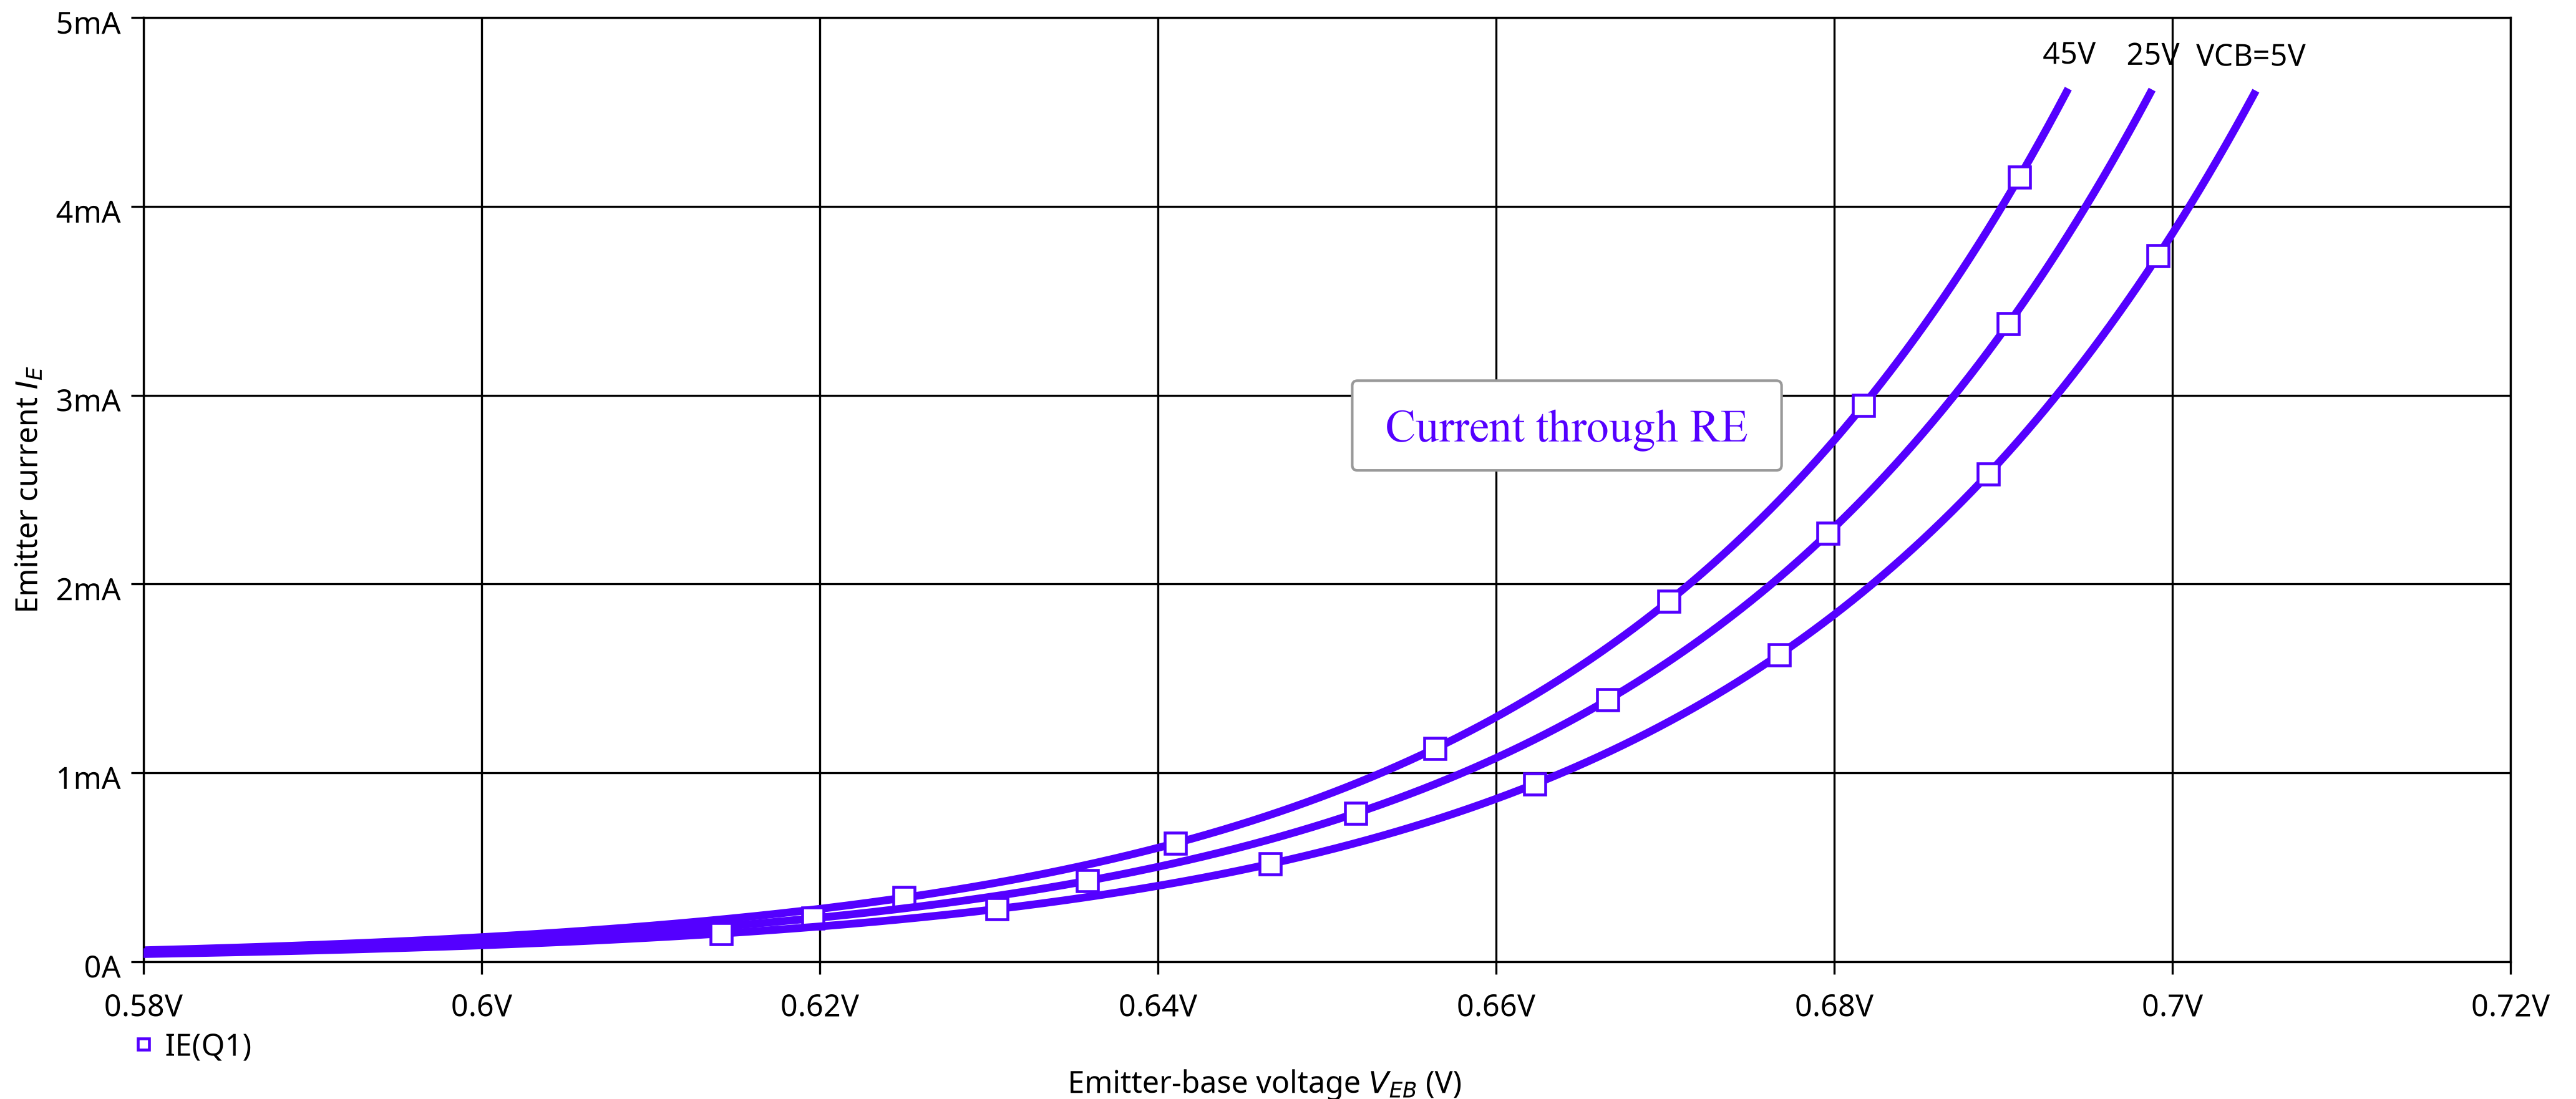
\includegraphics[width=\textwidth]{cb_input_npn.png}
		\caption{PSpice output: input characteristic of the NPN transistor in CB configuration for $V_{CC} = 5$, 25 and \SI{45}{\volt} ($V_{CB} \approx V_{CC}$). The current rises exponentially above the knee and reaches \SI{4.3}{\milli\ampere} at \SI{0.703}{\volt}; the \SI{45}{\volt} curve lies about \SI{10}{\milli\volt} to the left of the \SI{5}{\volt} curve through the Early effect.}
		\label{fig:cb-in-npn}
	\end{figure}
	
	\begin{figure}[H]
		\centering
		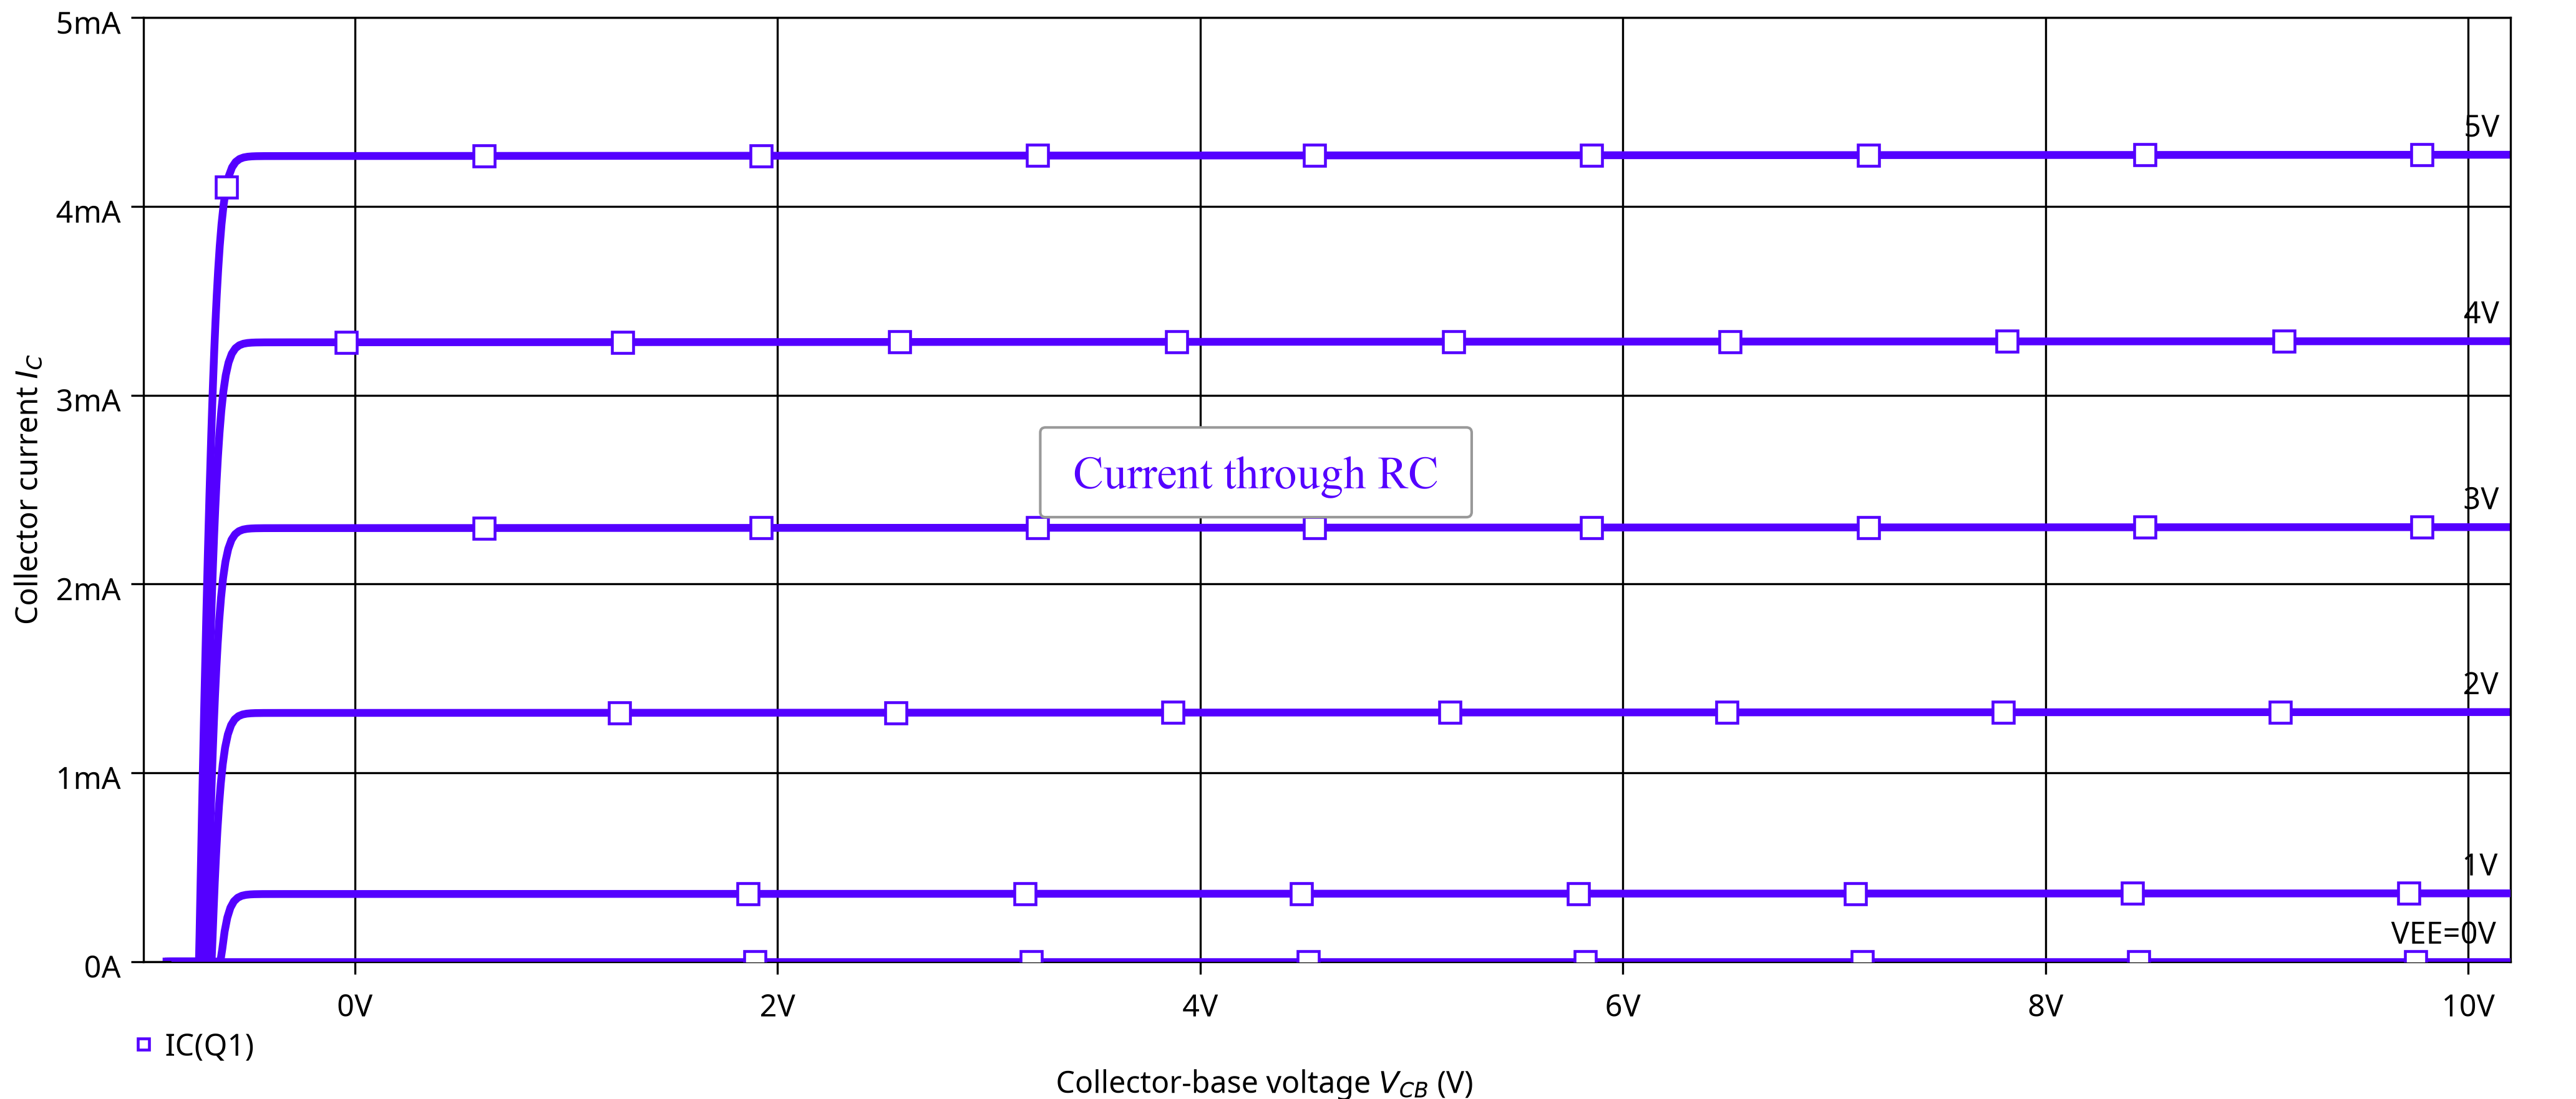
\includegraphics[width=\textwidth]{cb_output_npn.png}
		\caption{PSpice output: output characteristic of the NPN transistor in CB configuration for $V_{EE} = 0$ to \SI{5}{\volt}, i.e. $I_E \approx 0$ to \SI{4.3}{\milli\ampere}. The $V_{EE} = 0$ trace along the axis is the cutoff region, saturation lies at negative $V_{CB}$ with the knee at \SI{-0.63}{\volt}, and each active-region trace sits at $I_C \approx 0.994\,I_E$ with a small positive slope.}
		\label{fig:cb-out-npn}
	\end{figure}
	
	\begin{figure}[H]
		\centering
		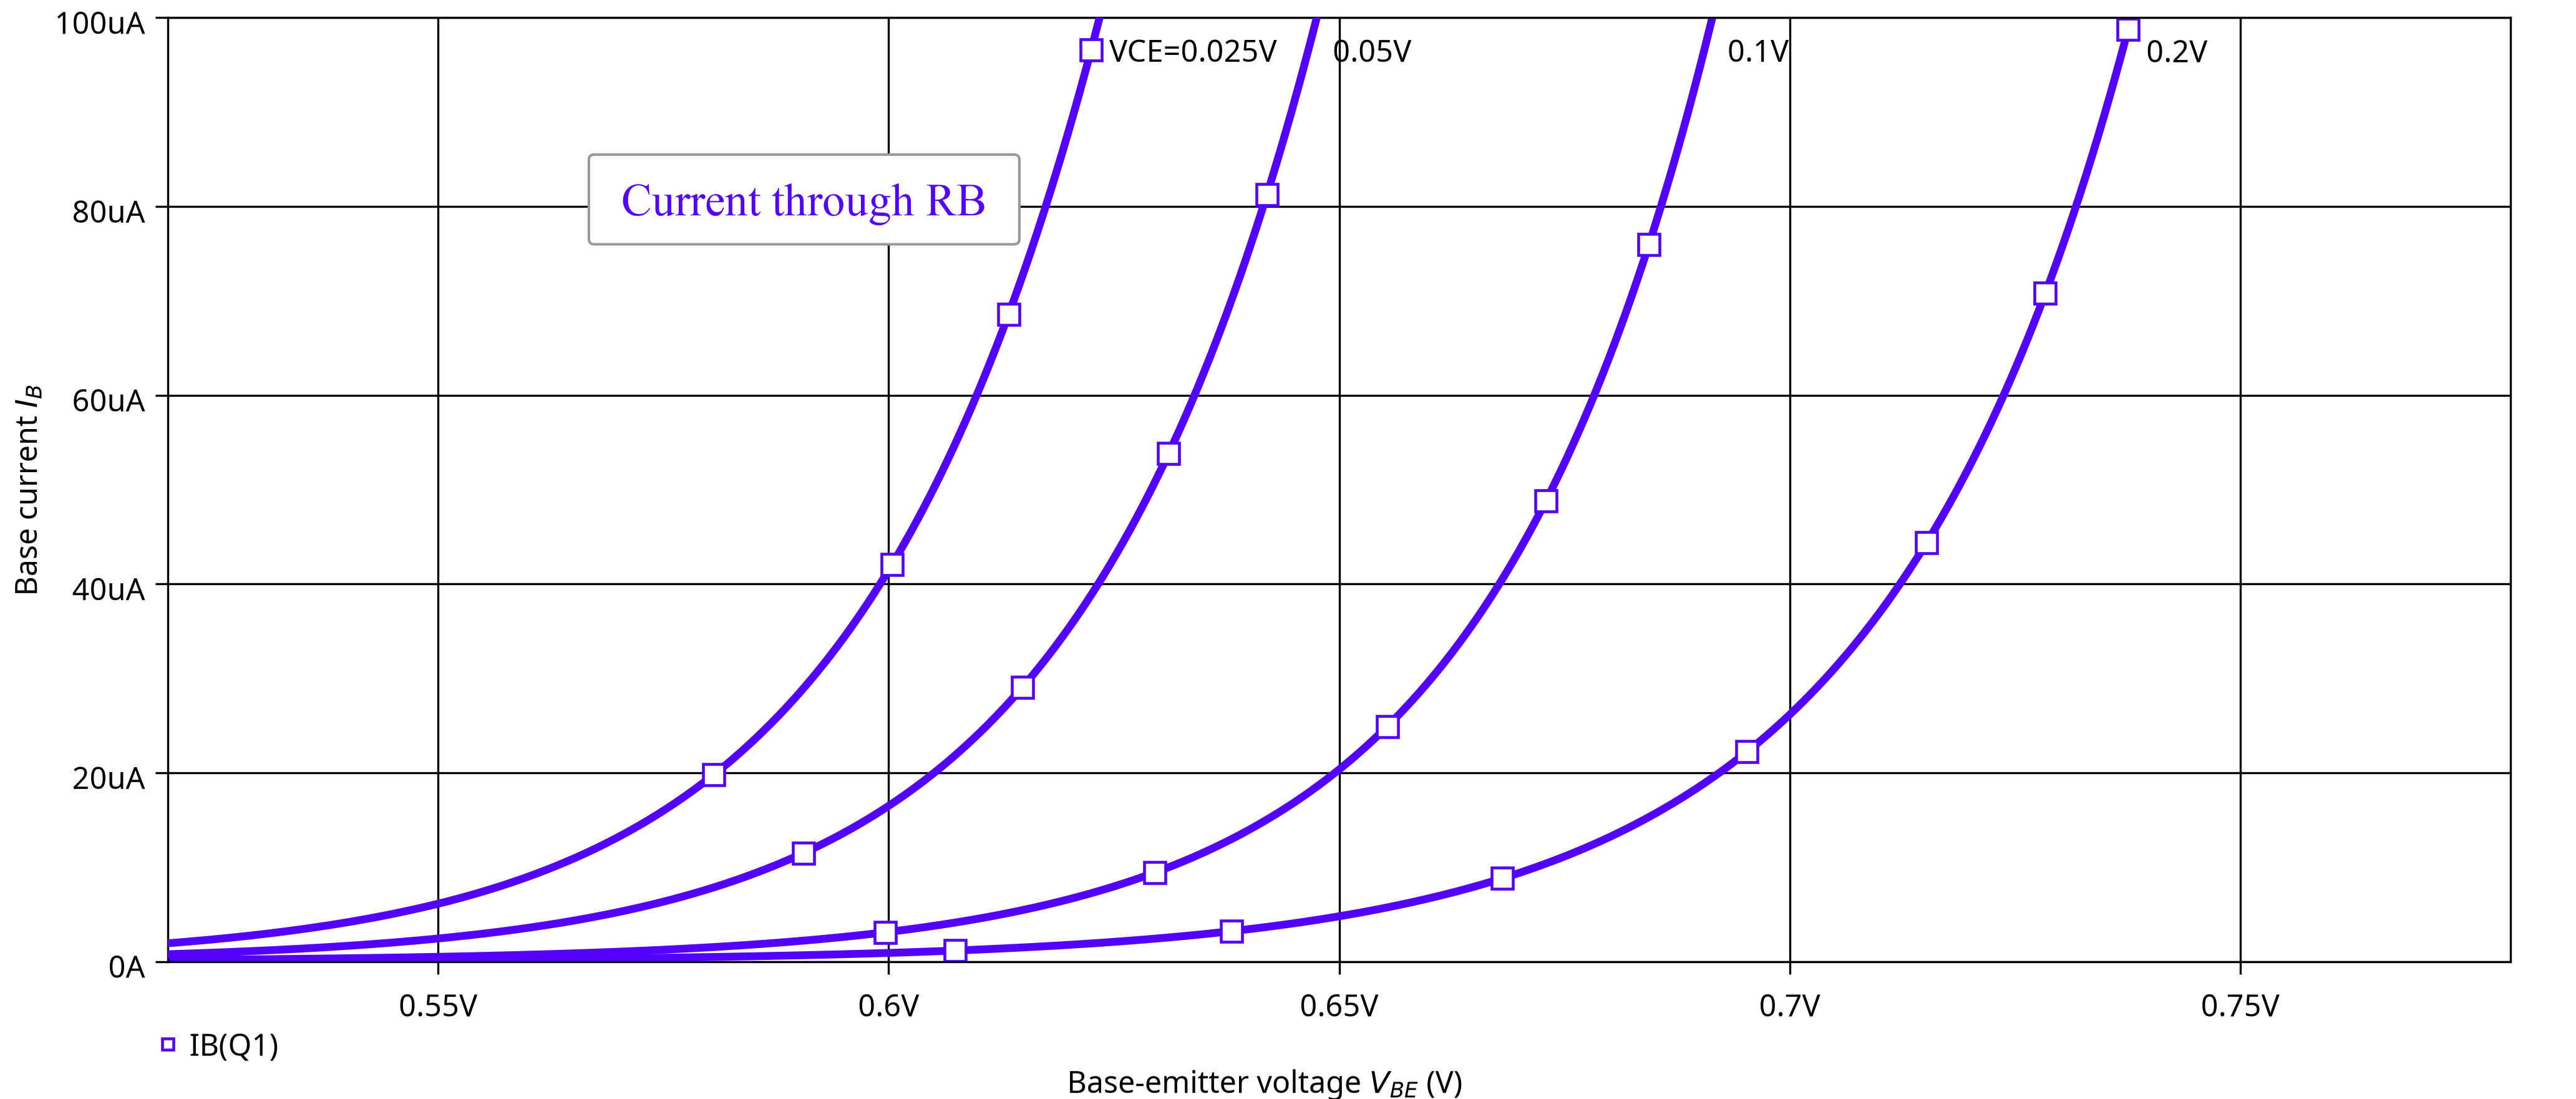
\includegraphics[width=\textwidth]{ce_input_npn.png}
		\caption{PSpice output: input characteristic of the NPN transistor in CE configuration for $V_{CC} = 0.025$, 0.05, 0.1 and \SI{0.2}{\volt} (octave sweep, $V_{CE} \approx V_{CC}$). The curves move to the right as $V_{CC}$ increases because the forward bias of the collector junction falls; above about \SI{0.3}{\volt} the curves for larger $V_{CC}$ would merge into one.}
		\label{fig:ce-in-npn}
	\end{figure}
	
	\begin{figure}[H]
		\centering
		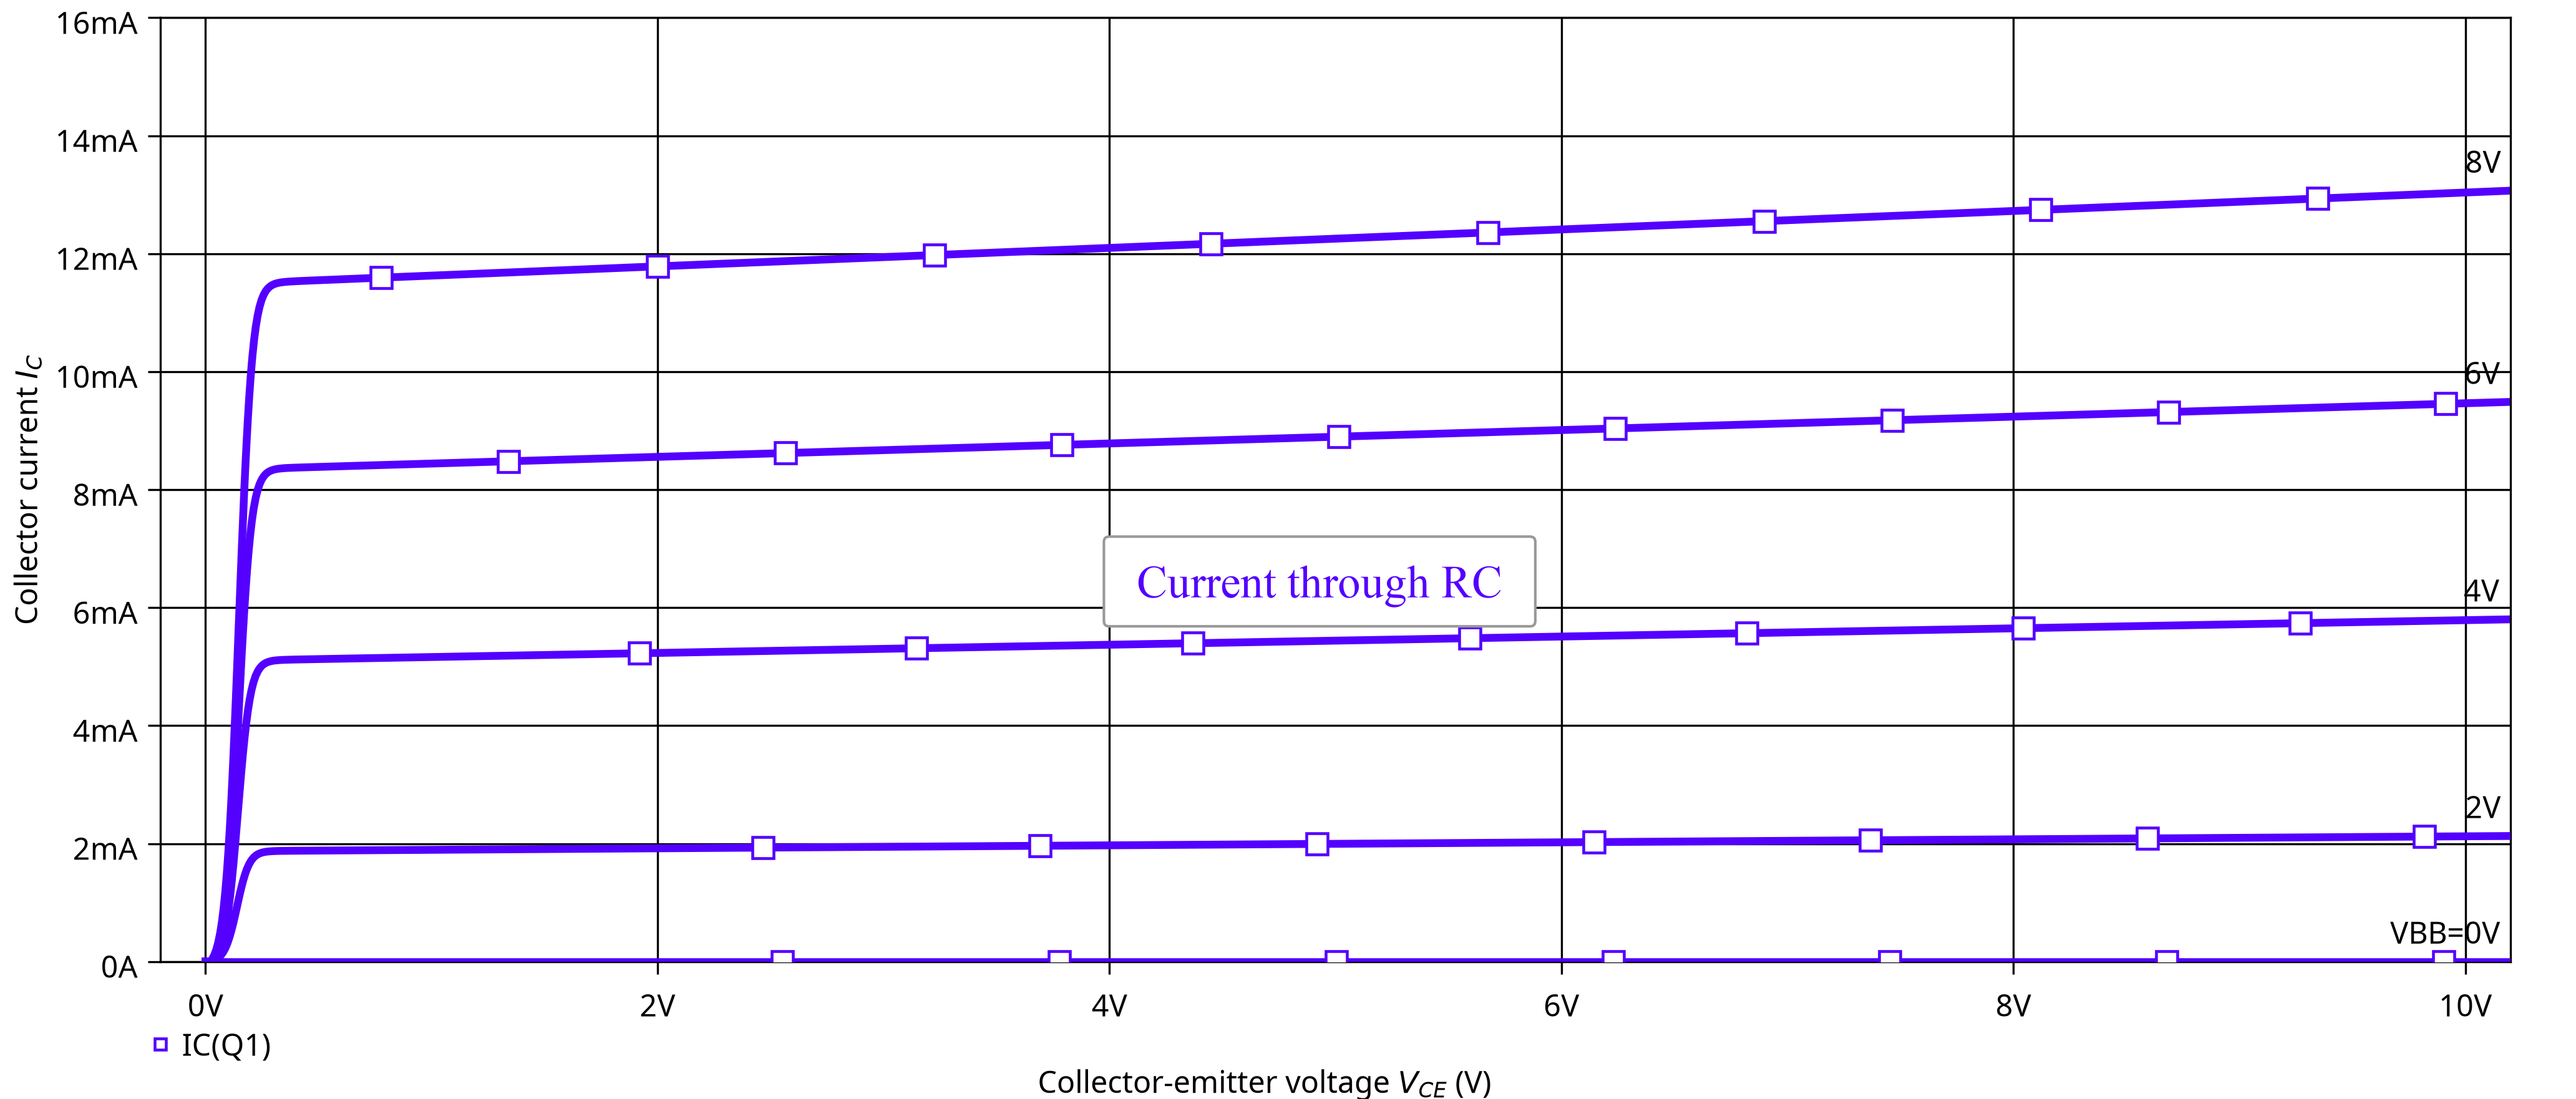
\includegraphics[width=\textwidth]{ce_output_npn.png}
		\caption{PSpice output: output characteristic of the NPN transistor in CE configuration for $V_{BB} = 0$ to \SI{8}{\volt} ($I_B \approx 0$ to \SI{73}{\micro\ampere}). The knee at \SI{0.21}{\volt} separates the saturation region from the active region, where the traces are spaced by about \SI{3.5}{\milli\ampere} per \SI{20}{\micro\ampere}; the $V_{BB} = 0$ trace is the cutoff region.}
		\label{fig:ce-out-npn}
	\end{figure}
	
	\begin{figure}[H]
		\centering
		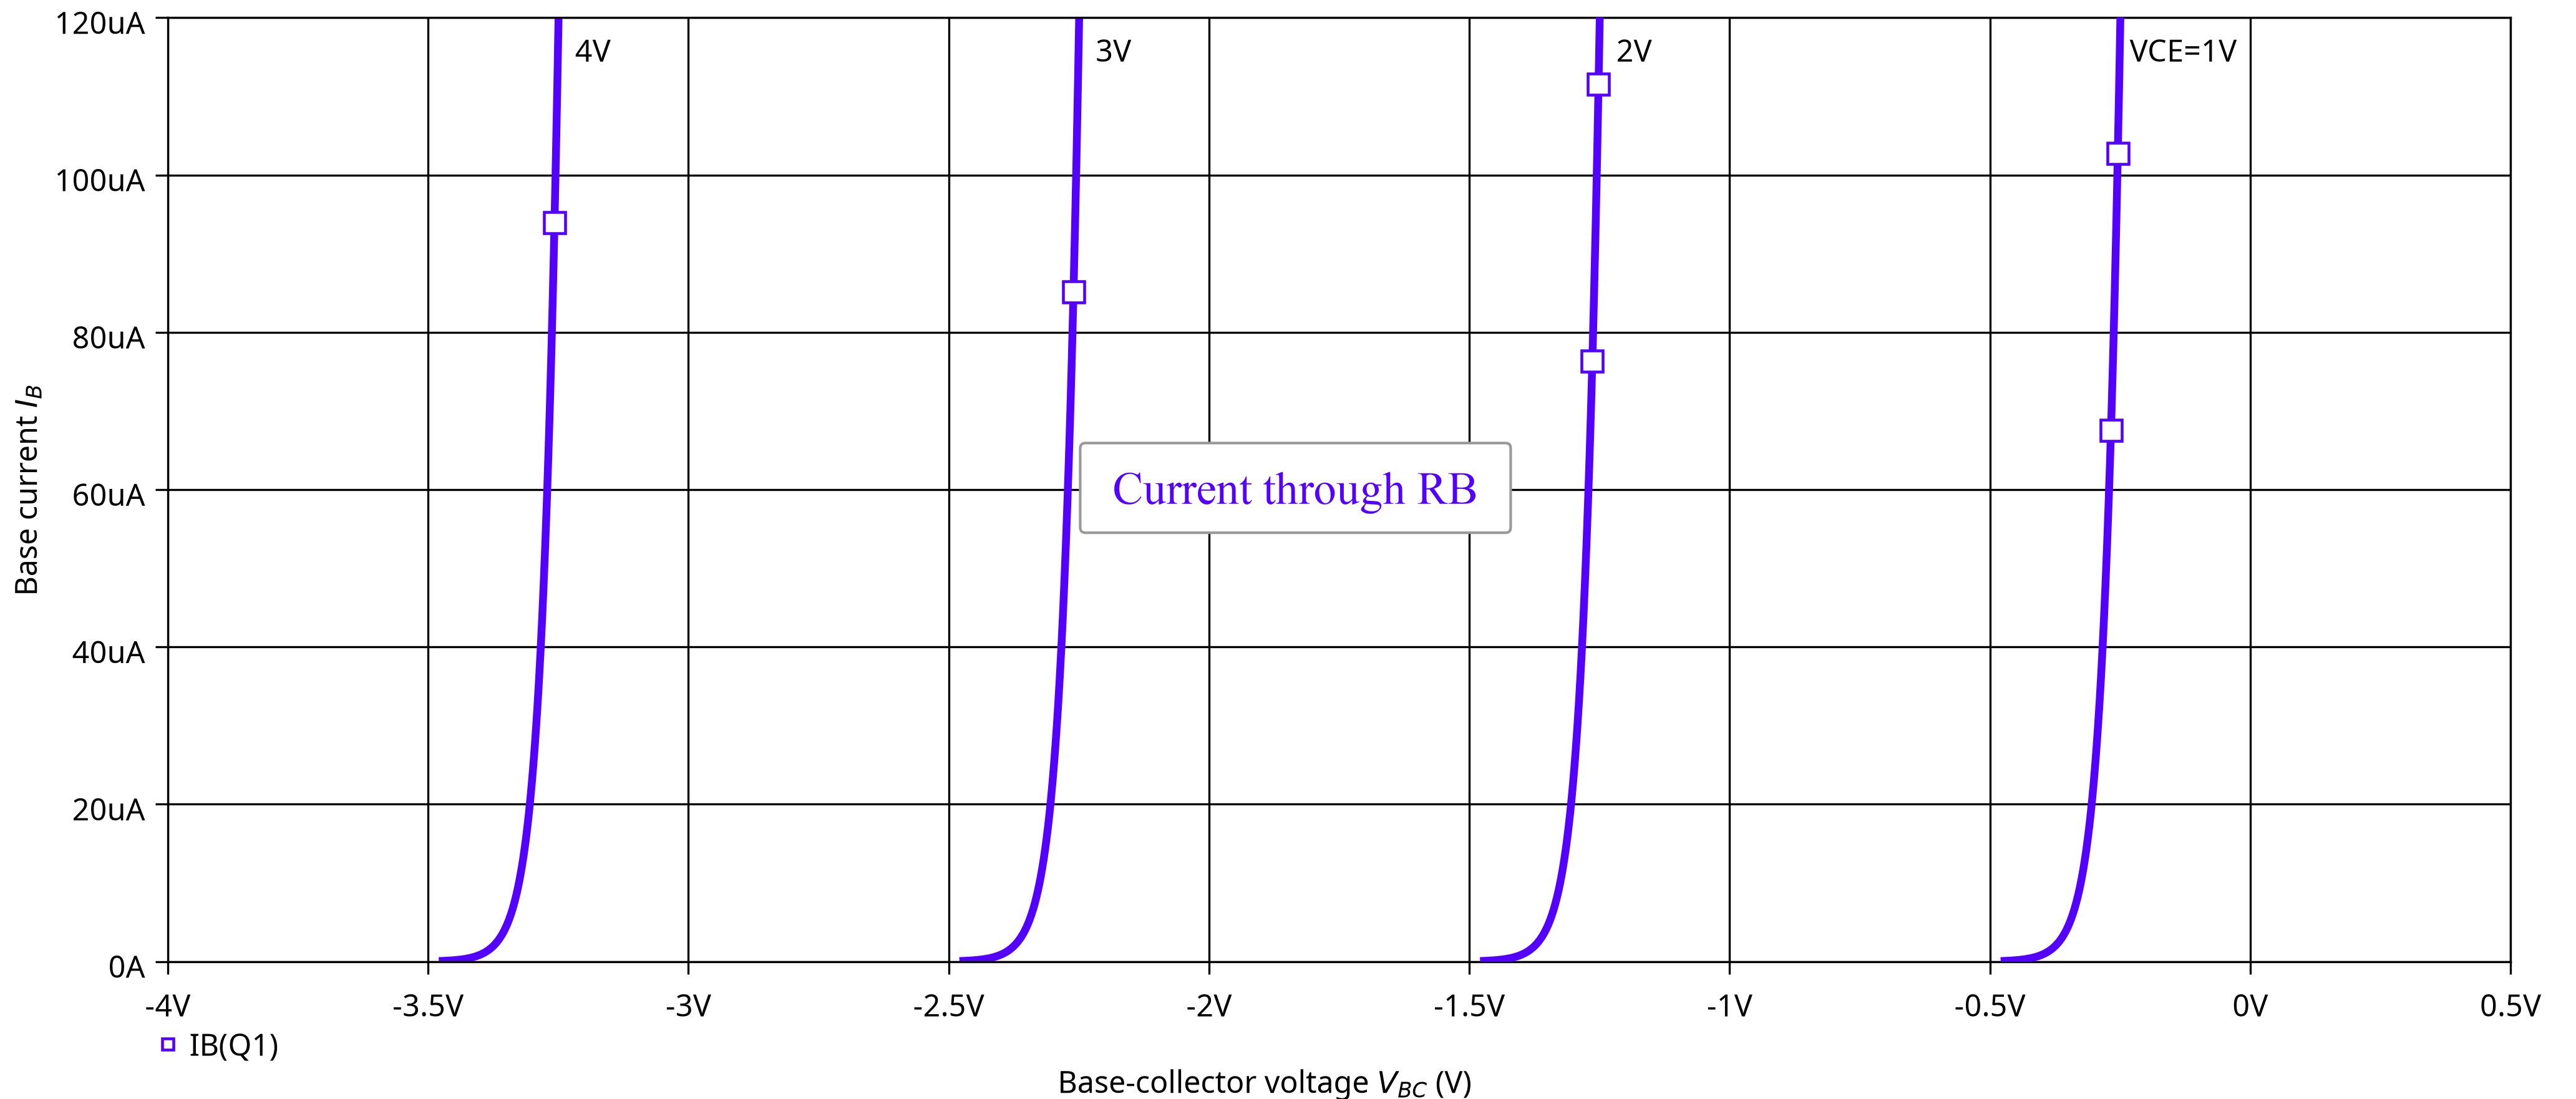
\includegraphics[width=\textwidth]{cc_input_npn.png}
		\caption{PSpice output: input characteristic of the NPN transistor in CC configuration for $V_{EE} = -1$, $-2$, $-3$ and \SI{-4}{\volt} ($V_{CE} = 1$, 2, 3 and \SI{4}{\volt}), plotted against $V_{BC}$. The curves are separated by about \SI{1}{\volt} because $V_{BC} = V_{BE} - V_{CE}$; the \SI{4}{\volt} curve is the leftmost.}
		\label{fig:cc-in-npn}
	\end{figure}
	
	\begin{figure}[H]
		\centering
		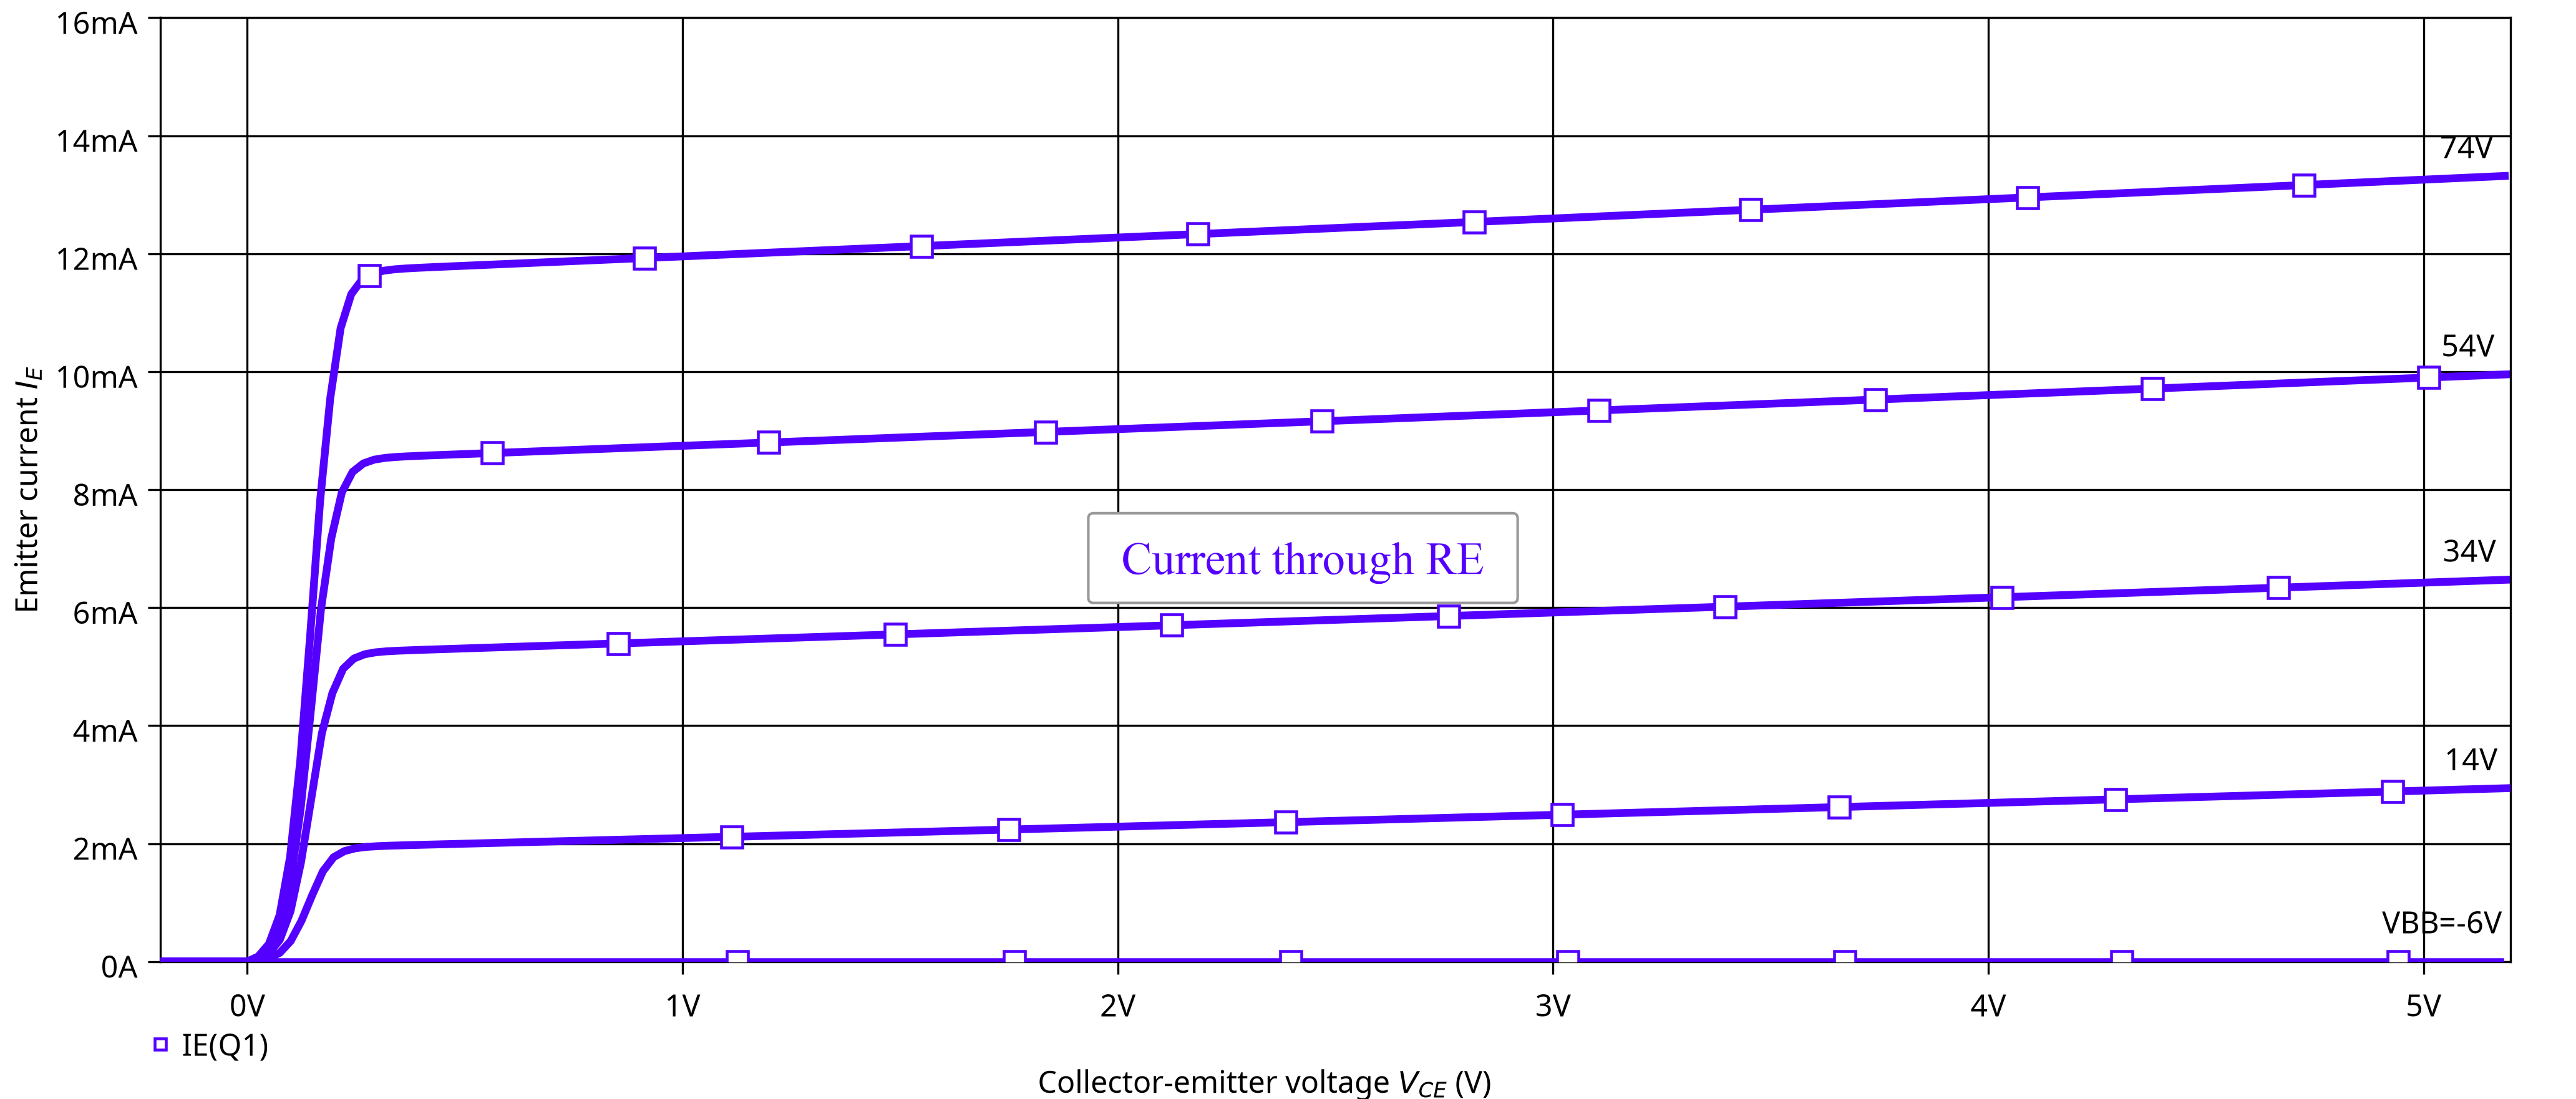
\includegraphics[width=\textwidth]{cc_output_npn.png}
		\caption{PSpice output: output characteristic of the NPN transistor in CC configuration for $V_{BB} = -6$, 14, 34, 54 and \SI{74}{\volt} ($I_B \approx 0$ to \SI{74}{\micro\ampere}). The knee at \SI{0.22}{\volt} separates saturation from the active region, and the emitter current is the largest terminal current, about one base current above the corresponding CE value.}
		\label{fig:cc-out-npn}
	\end{figure}
	
	The CB input characteristic of Figure~\ref{fig:cb-in-npn} shows the
	exponential behavior of \eqref{eq:shockley}: the emitter current is below
	\SI{0.1}{\milli\ampere} at \SI{0.58}{\volt}, reaches
	\SI{3.30}{\milli\ampere} at \SI{0.696}{\volt} and \SI{4.30}{\milli\ampere}
	at \SI{0.703}{\volt}. The \SI{45}{\volt} curve is displaced to the left
	of the \SI{5}{\volt} curve by about \SI{10}{\milli\volt}, which is the
	Early shift over a forty-volt span. The chord slope between the two
	readings gives the \SI{7.242}{\ohm} input resistance, close to the
	\SI{6.841}{\ohm} calculated in Section~\ref{sec:calc}. The CB output
	family of Figure~\ref{fig:cb-out-npn} falls steeply for $V_{CB}$ below
	\SI{-0.63}{\volt}, where the collector junction is forward biased and the
	device is saturated, and levels off at $I_C \approx 0.994\,I_E$ once
	$V_{CB}$ is above that knee. In the active region the highest trace rises
	by \SI{3.08}{\micro\ampere} between \SI{5}{\volt} and \SI{10}{\volt},
	and after the small drift of $I_E$ is removed this slope gives
	$R_{\mathrm{out,CB}} = \SI{3.497}{\mega\ohm}$. The nearly horizontal
	traces also show that the CB connection delivers almost the whole emitter
	current to the collector, since $\alpha$ differs from unity by only a few
	parts per thousand.
	
	The CE input family of Figure~\ref{fig:ce-in-npn} is taken at the edge of
	saturation, where $V_{CC}$, and with it $V_{CE}$, runs from 0.025 to
	\SI{0.2}{\volt}. At these voltages the collector junction is forward
	biased and its current adds to the base current, so the curves move to
	the right as $V_{CC}$ increases, opposite to the small Early shift of the
	active region; above about \SI{0.3}{\volt} the base current no longer
	depends on $V_{CE}$ and the curves for larger $V_{CC}$, such as the
	\SI{5}{\volt} reference run, lie on top of each other.
	On the $V_{CC} = \SI{5}{\volt}$ reference curve the base current reaches
	\SI{32.90}{\micro\ampere} at \SI{0.710}{\volt} and
	\SI{52.76}{\micro\ampere} at \SI{0.724}{\volt}, so the input resistance is
	\SI{708.5}{\ohm}, about one hundred times the CB value. The CE output
	family of Figure~\ref{fig:ce-out-npn} shows the saturation knee at
	\SI{0.21}{\volt}, then almost flat traces spaced by about
	\SI{3.5}{\milli\ampere} per \SI{20}{\micro\ampere} of base current. The
	collector current reaches \SI{8.897}{\milli\ampere} at
	$V_{CE} = \SI{5}{\volt}$ for $I_B = \SI{52.76}{\micro\ampere}$, giving
	$\beta = 174.0$, and the upward slope between \SI{5}{\volt} and
	\SI{10}{\volt} gives $R_{\mathrm{out,CE}} = \SI{8.801}{\kilo\ohm}$.
	Since $V_{CE} = V_{CB} + V_{BE}$, the CB knee at
	$V_{CB} \approx \SI{-0.63}{\volt}$ and a base-emitter voltage of about
	\SI{0.72}{\volt} correspond to $V_{CE} \approx \SI{0.1}{\volt}$, the same
	order as the \SI{0.21}{\volt} knee read from
	Figure~\ref{fig:ce-out-npn}; the remaining difference of about
	\SI{0.1}{\volt} depends on the trace current and on the \SI{90}{\percent}
	criterion used to read the knee.
	
	The CC input family of Figure~\ref{fig:cc-in-npn} is plotted against
	$V_{BC}$, so the four curves are separated by about \SI{1}{\volt} of
	$V_{CE}$ because $V_{BC} = V_{BE} - V_{CE}$. At $V_{CE} = \SI{4}{\volt}$
	the base current rises from \SI{38.29}{\micro\ampere} to
	\SI{58.27}{\micro\ampere} as $V_{BC}$ goes from \SI{-3.2849}{\volt} to
	\SI{-3.2720}{\volt}, which gives $R_{\mathrm{in,CC}} =
	\SI{645.4}{\ohm}$; this is close to, but not identical with, the CE value
	because the two families are read at different base currents. In the CC
	output family of Figure~\ref{fig:cc-out-npn} the ordinate is the emitter
	current, so each trace lies about one base current above the CE trace at
	the same base current. At $V_{CE} = \SI{5}{\volt}$ the emitter current
	rises from \SI{6.424}{\milli\ampere} to \SI{9.897}{\milli\ampere} as
	$I_B$ goes from \SI{38.29}{\micro\ampere} to
	\SI{58.27}{\micro\ampere}, which gives $\gamma = 173.8$. This agrees with
	the measured $\beta$ to within \SI{0.2}{\percent} instead of exceeding
	it by one, because the two gains are read at different base currents
	(Section~\ref{sec:calc}). After the drift of $I_B$ along the trace is
	removed with $\Delta I_E - \gamma\,\Delta I_B$, the rise between
	\SI{3}{\volt} and \SI{5}{\volt} gives
	$R_{\mathrm{out,CC}} = \SI{8.418}{\kilo\ohm}$. The
	output characteristic confirms that the CC connection has an output
	resistance of the same order as the CE connection, while its output
	current is larger by the base current.
	
	\begin{figure}[H]
		\centering
		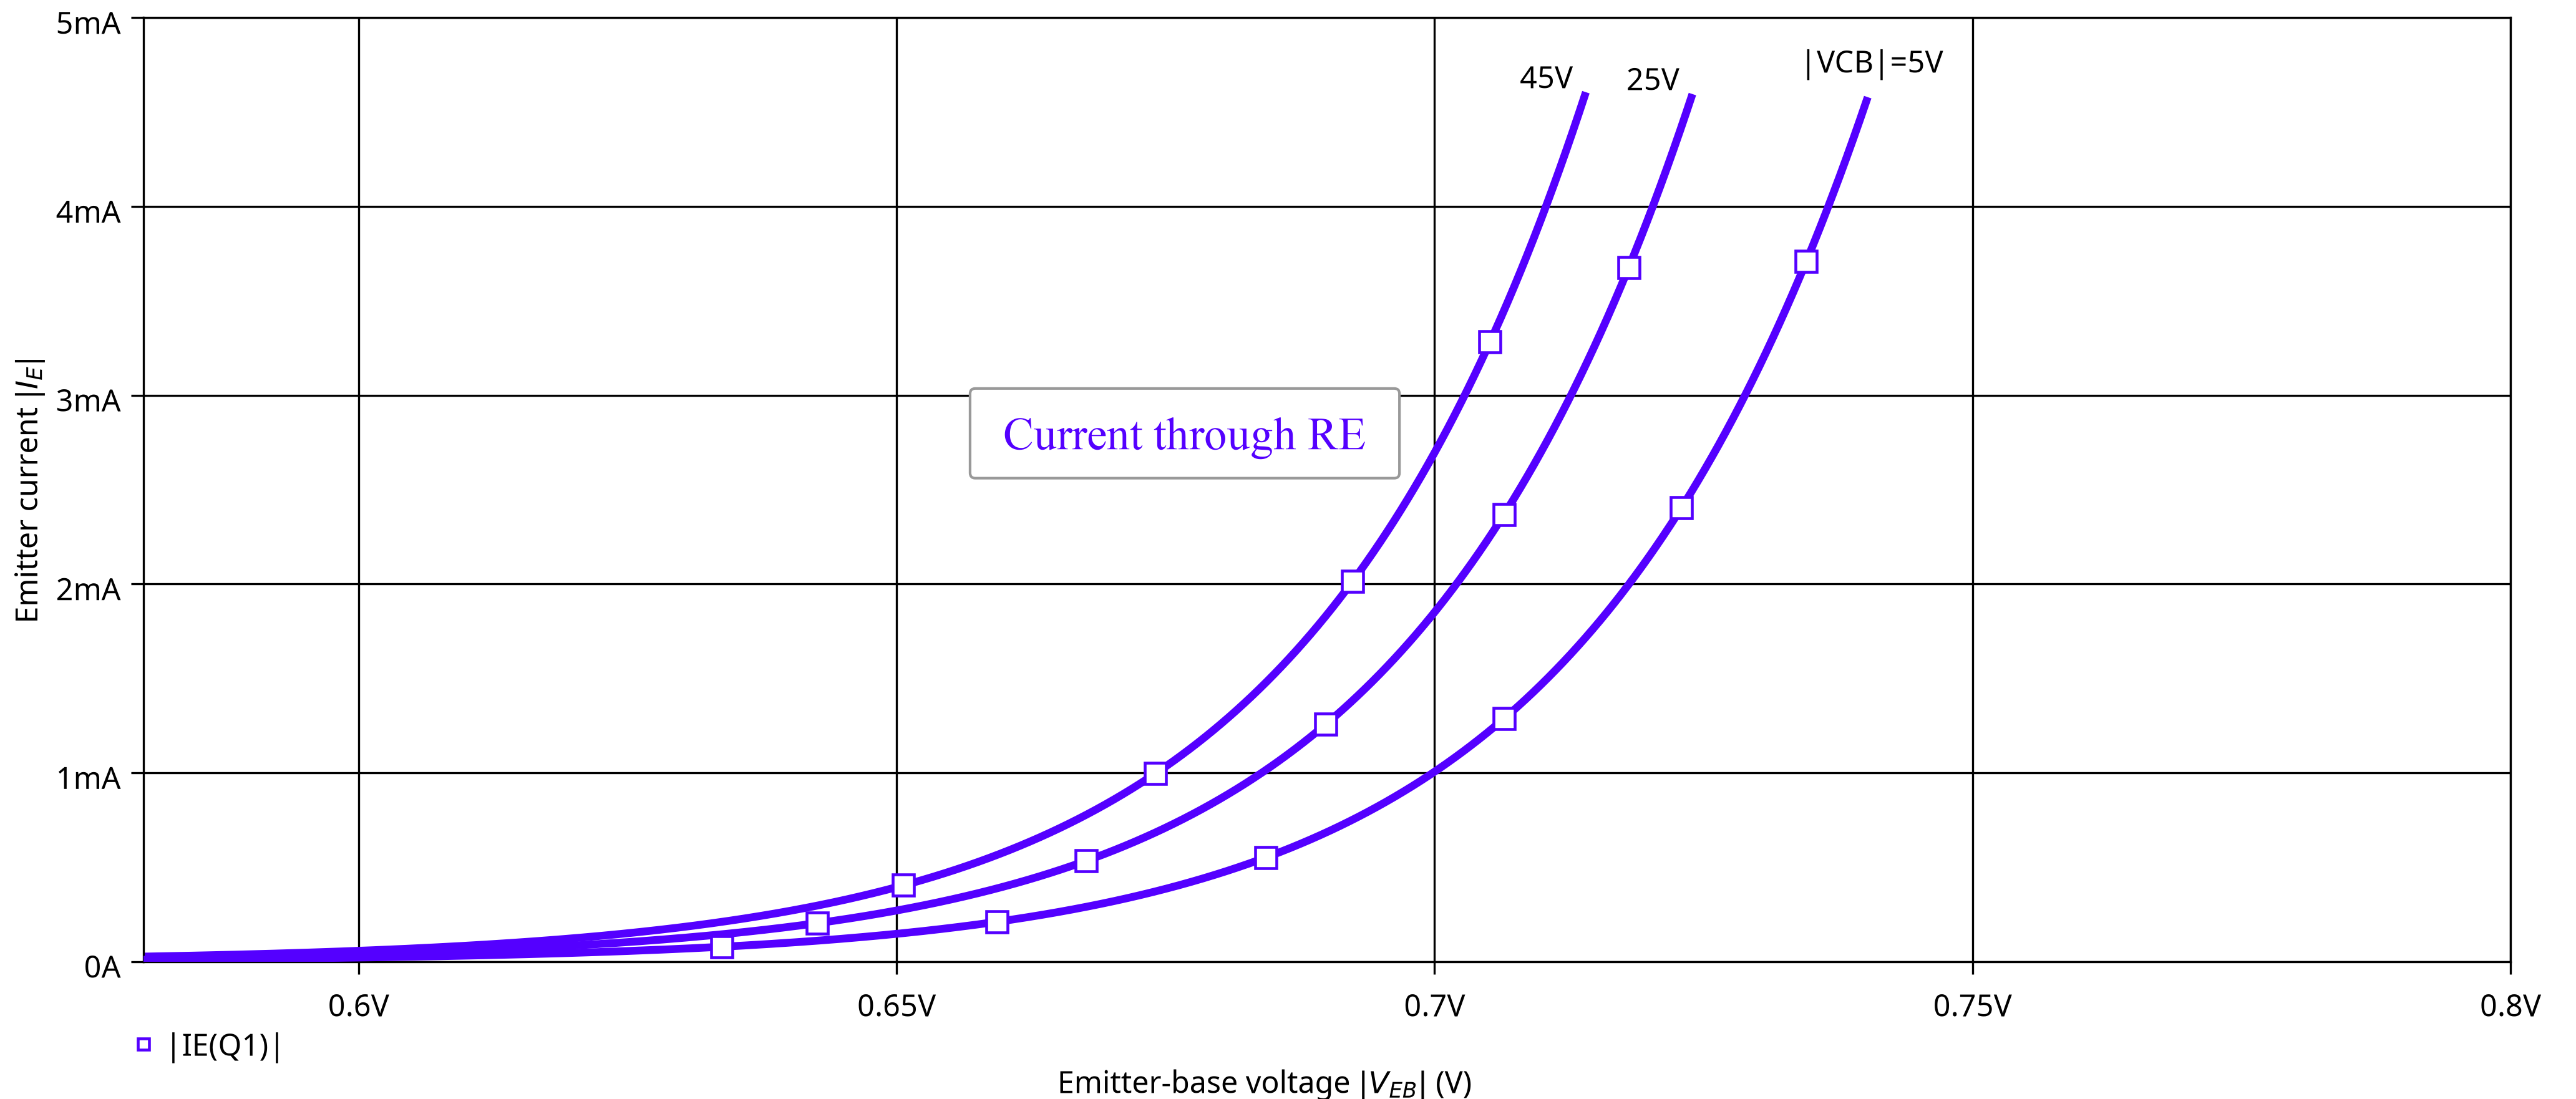
\includegraphics[width=\textwidth]{cb_input_pnp.png}
		\caption{PSpice output: input characteristic of the PNP transistor in CB configuration for $|V_{CC}| = 5$, 25 and \SI{45}{\volt}. The curve is the mirror image of Figure~\ref{fig:cb-in-npn} and the Early shift is larger, about \SI{25}{\milli\volt}, because the PNP Early voltage is only \SI{18.7}{\volt}.}
		\label{fig:cb-in-pnp}
	\end{figure}
	
	\begin{figure}[H]
		\centering
		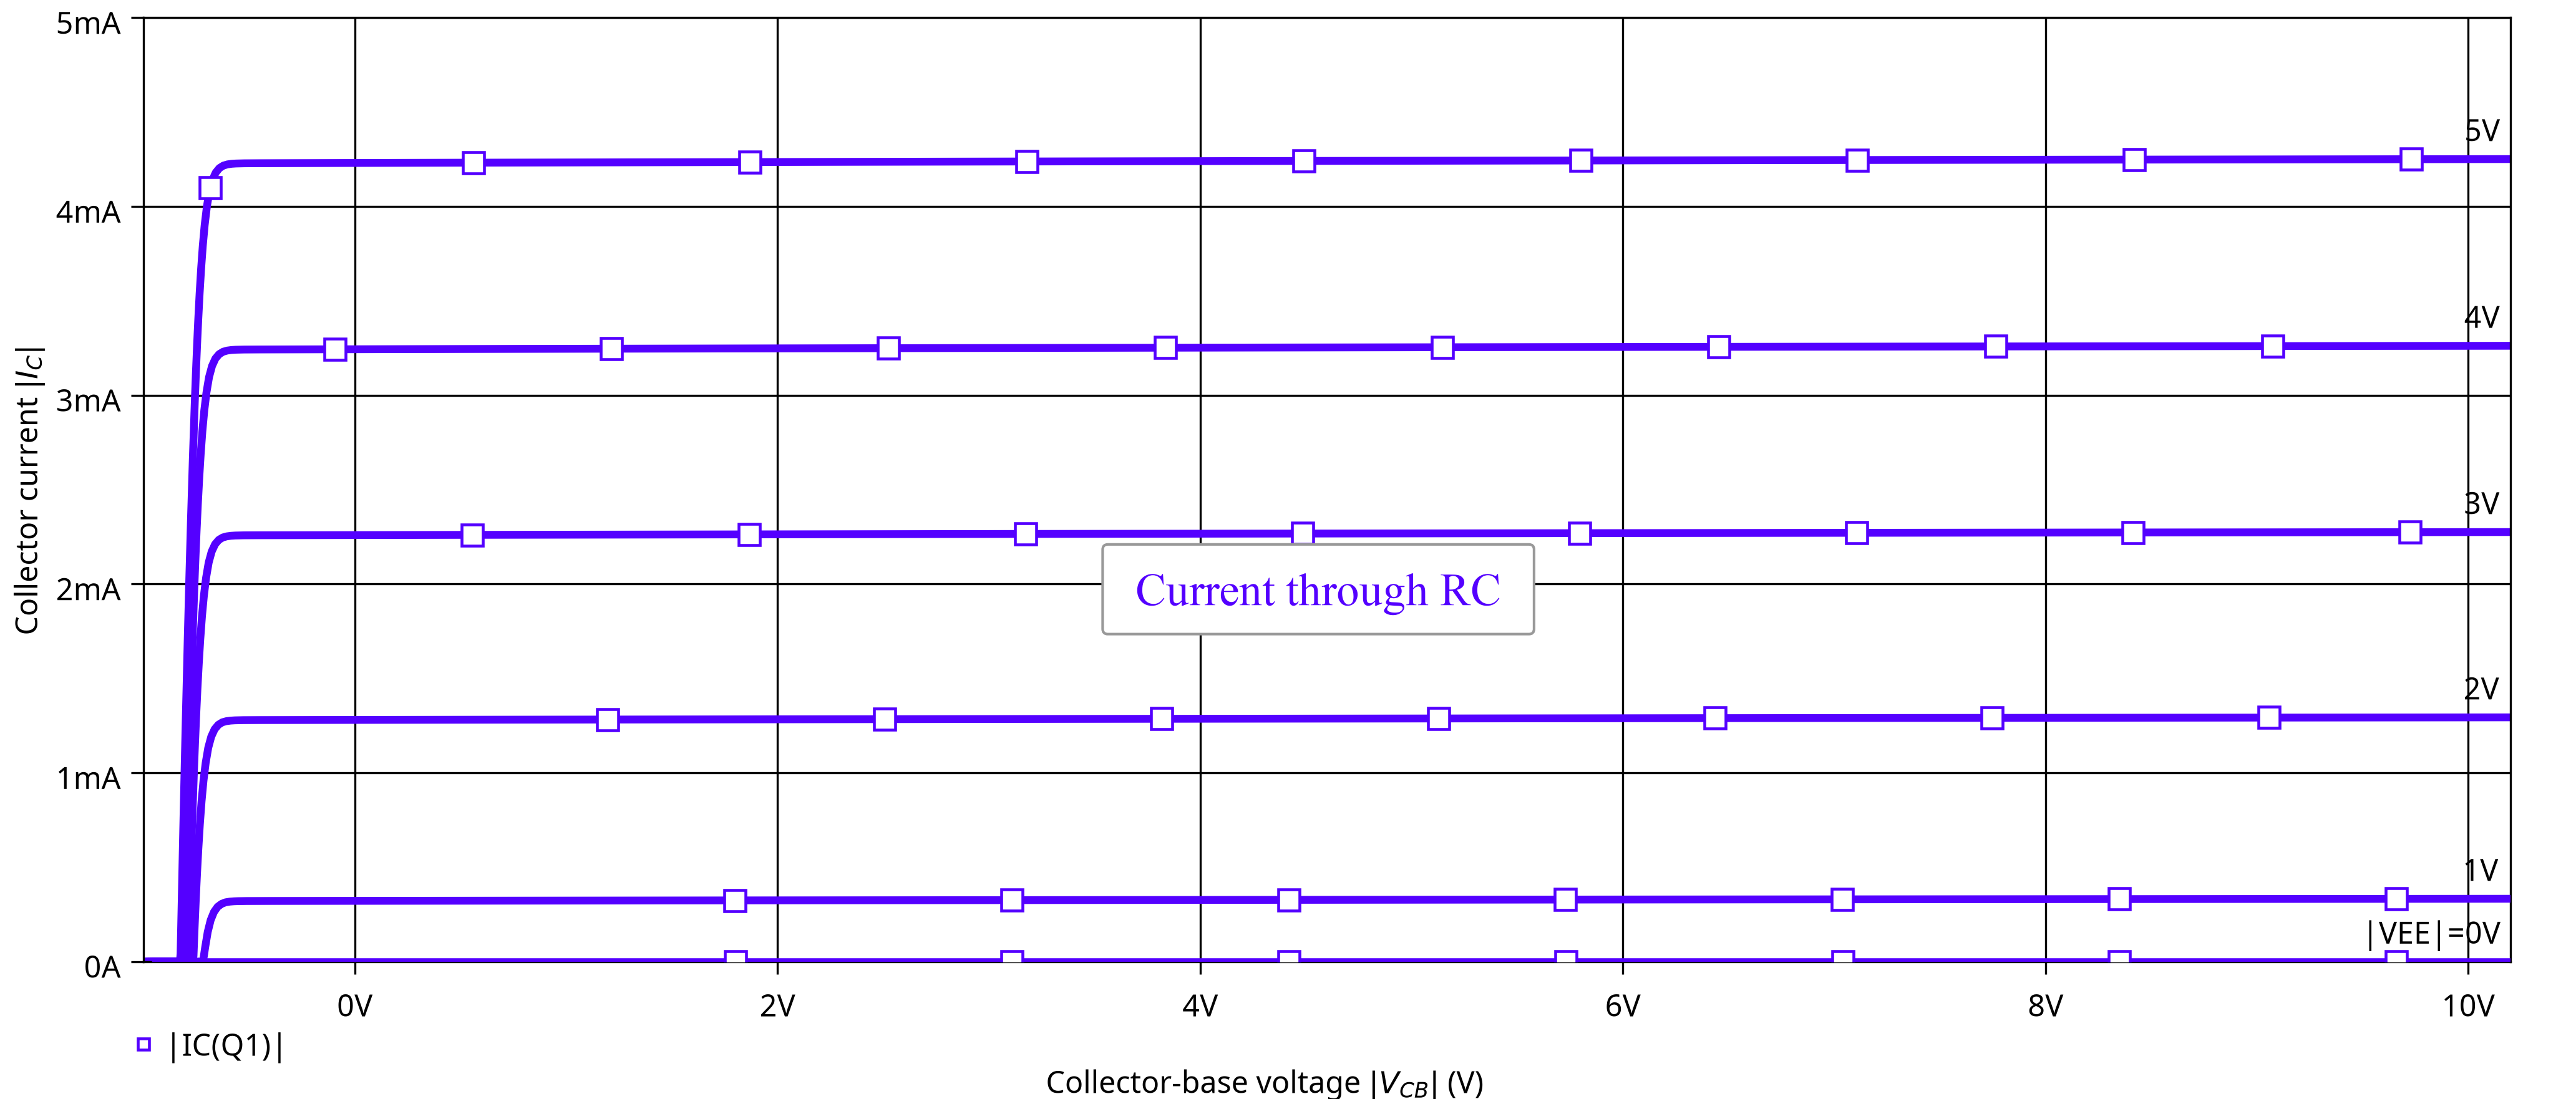
\includegraphics[width=\textwidth]{cb_output_pnp.png}
		\caption{PSpice output: output characteristic of the PNP transistor in CB configuration for $|V_{EE}| = 0$ to \SI{5}{\volt}. The saturation knee is at \SI{-0.71}{\volt} in the plotted coordinate and the active traces rise more steeply than for the NPN, because the PNP Early voltage is only \SI{18.7}{\volt}.}
		\label{fig:cb-out-pnp}
	\end{figure}
	
	\begin{figure}[H]
		\centering
		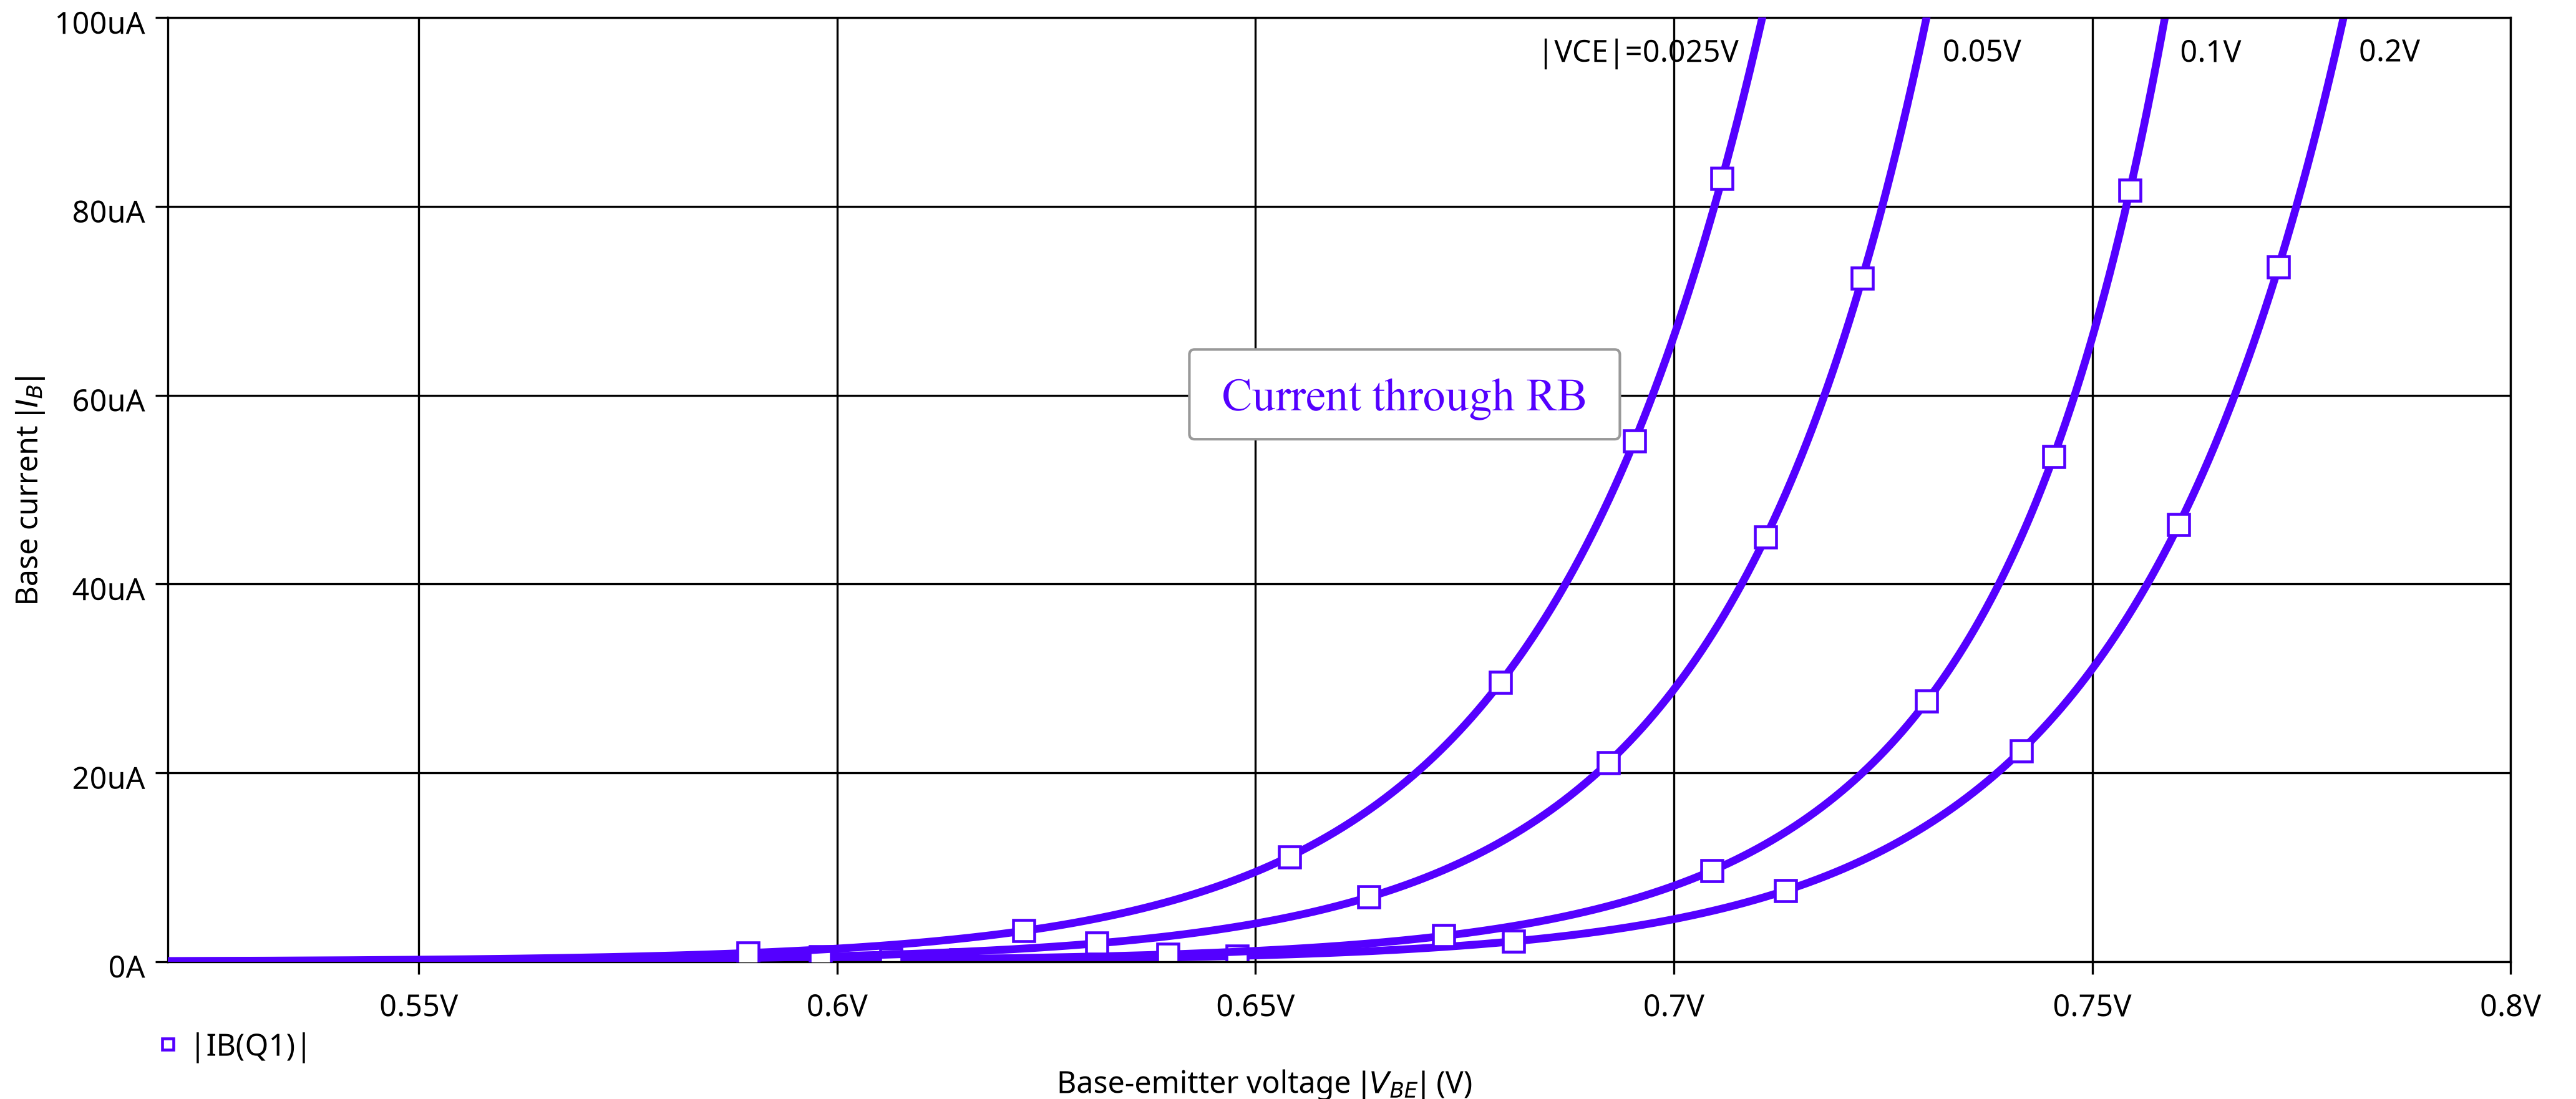
\includegraphics[width=\textwidth]{ce_input_pnp.png}
		\caption{PSpice output: input characteristic of the PNP transistor in CE configuration for $|V_{CC}| = 0.025$ to \SI{0.2}{\volt} (octave sweep, $|V_{CE}| \approx |V_{CC}|$). The curves spread to the right with increasing $|V_{CC}|$ in the same way as for the NPN.}
		\label{fig:ce-in-pnp}
	\end{figure}
	
	\begin{figure}[H]
		\centering
		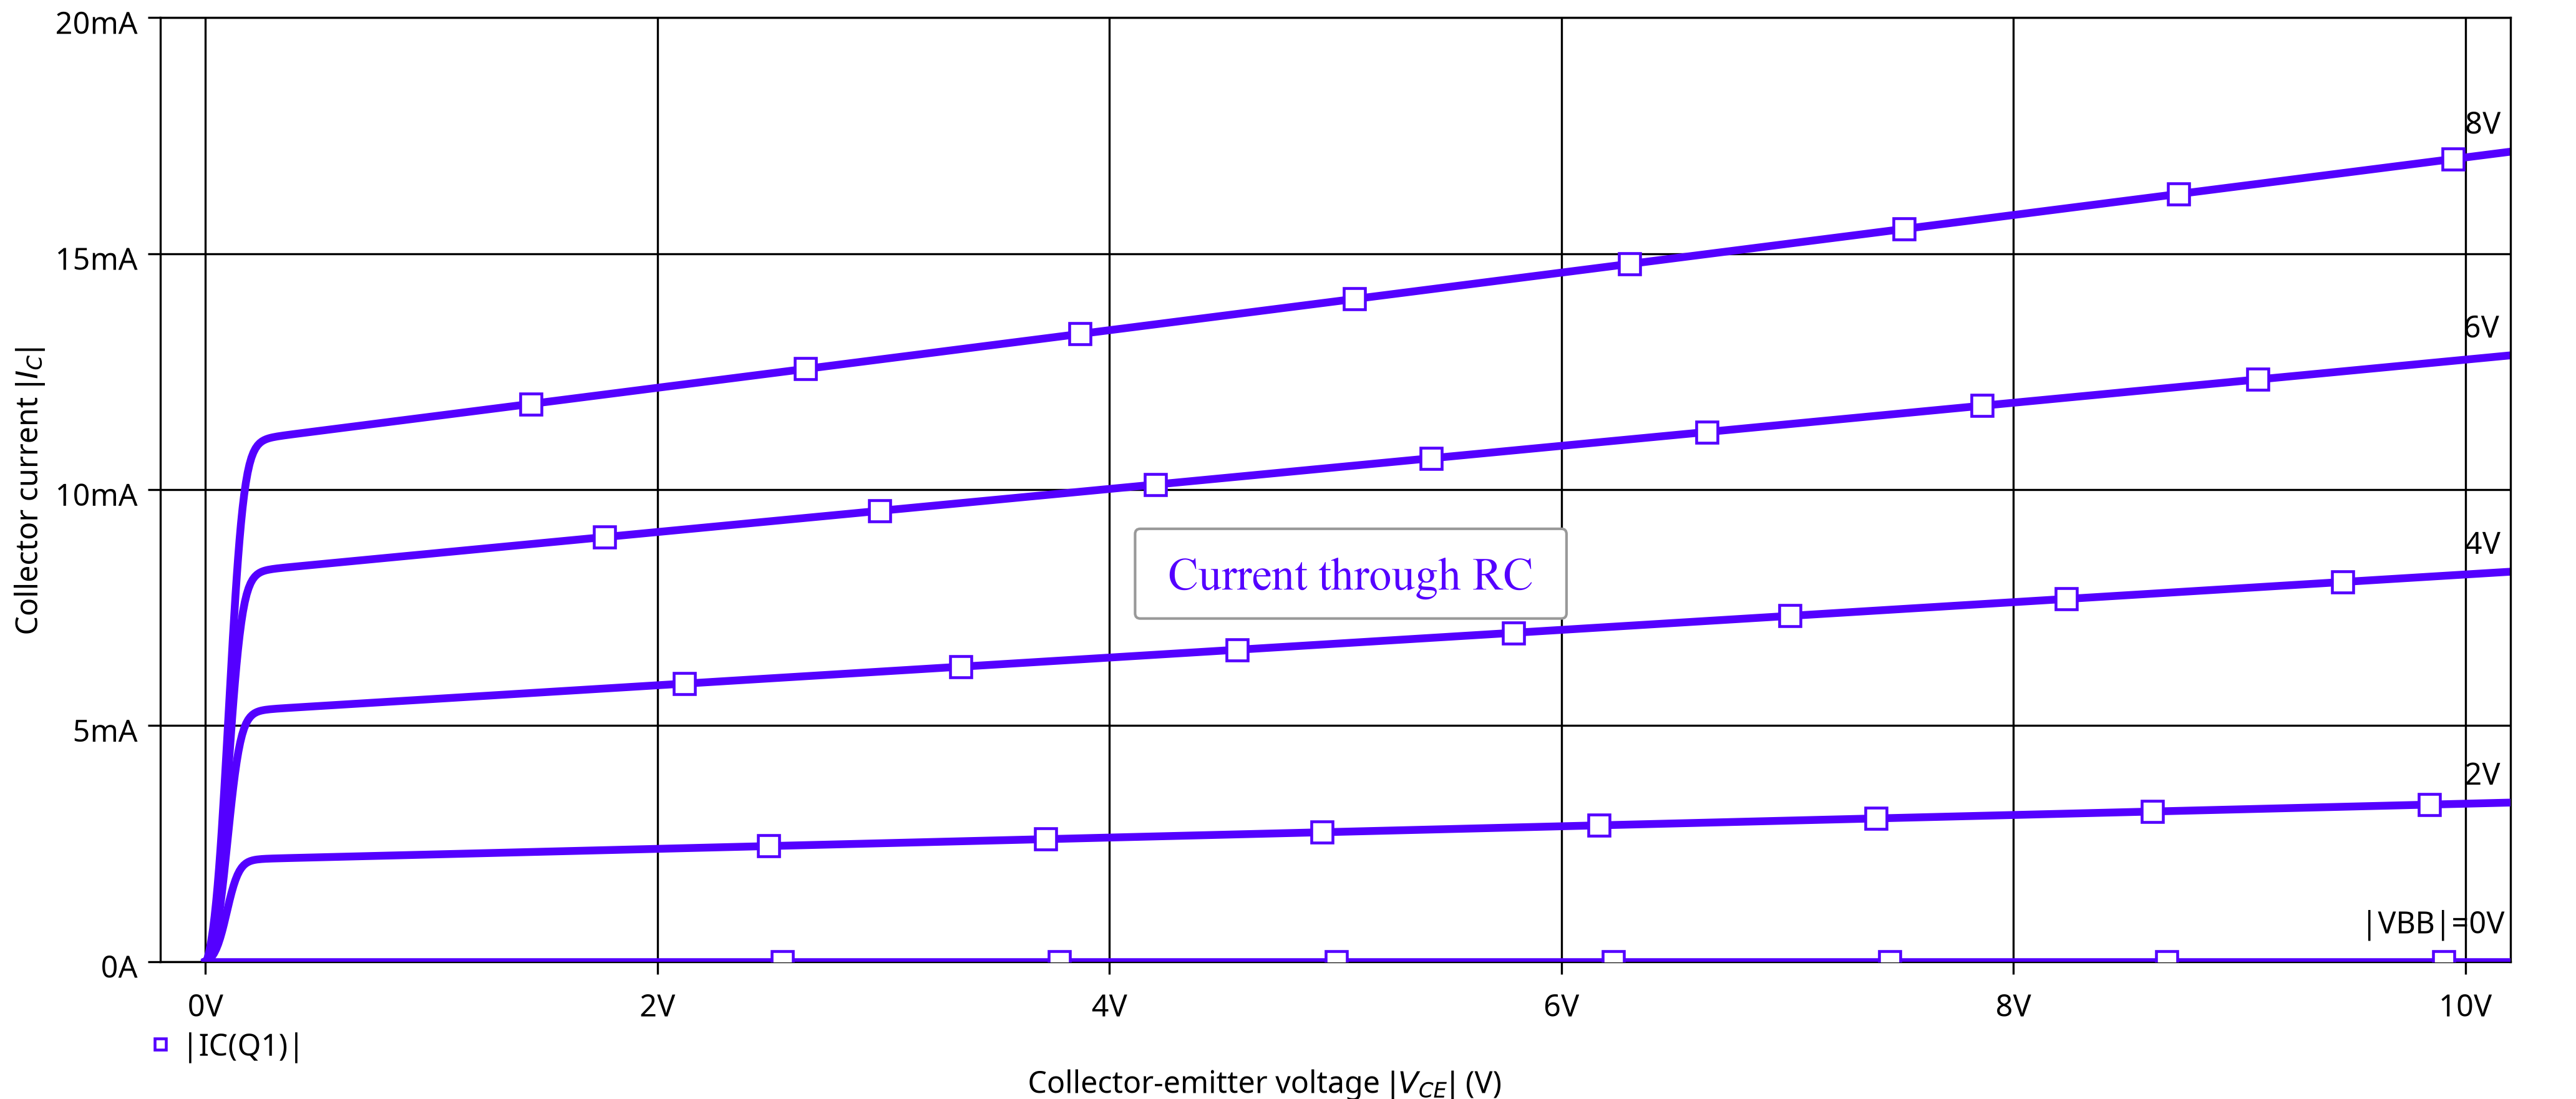
\includegraphics[width=\textwidth]{ce_output_pnp.png}
		\caption{PSpice output: output characteristic of the PNP transistor in CE configuration for $|V_{BB}| = 0$ to \SI{8}{\volt} ($|I_B| \approx 0$ to \SI{73}{\micro\ampere}). The spacing is about \SI{3.7}{\milli\ampere} per \SI{20}{\micro\ampere}, somewhat wider than the NPN spacing, and the traces rise more visibly with $|V_{CE}|$.}
		\label{fig:ce-out-pnp}
	\end{figure}
	
	\begin{figure}[H]
		\centering
		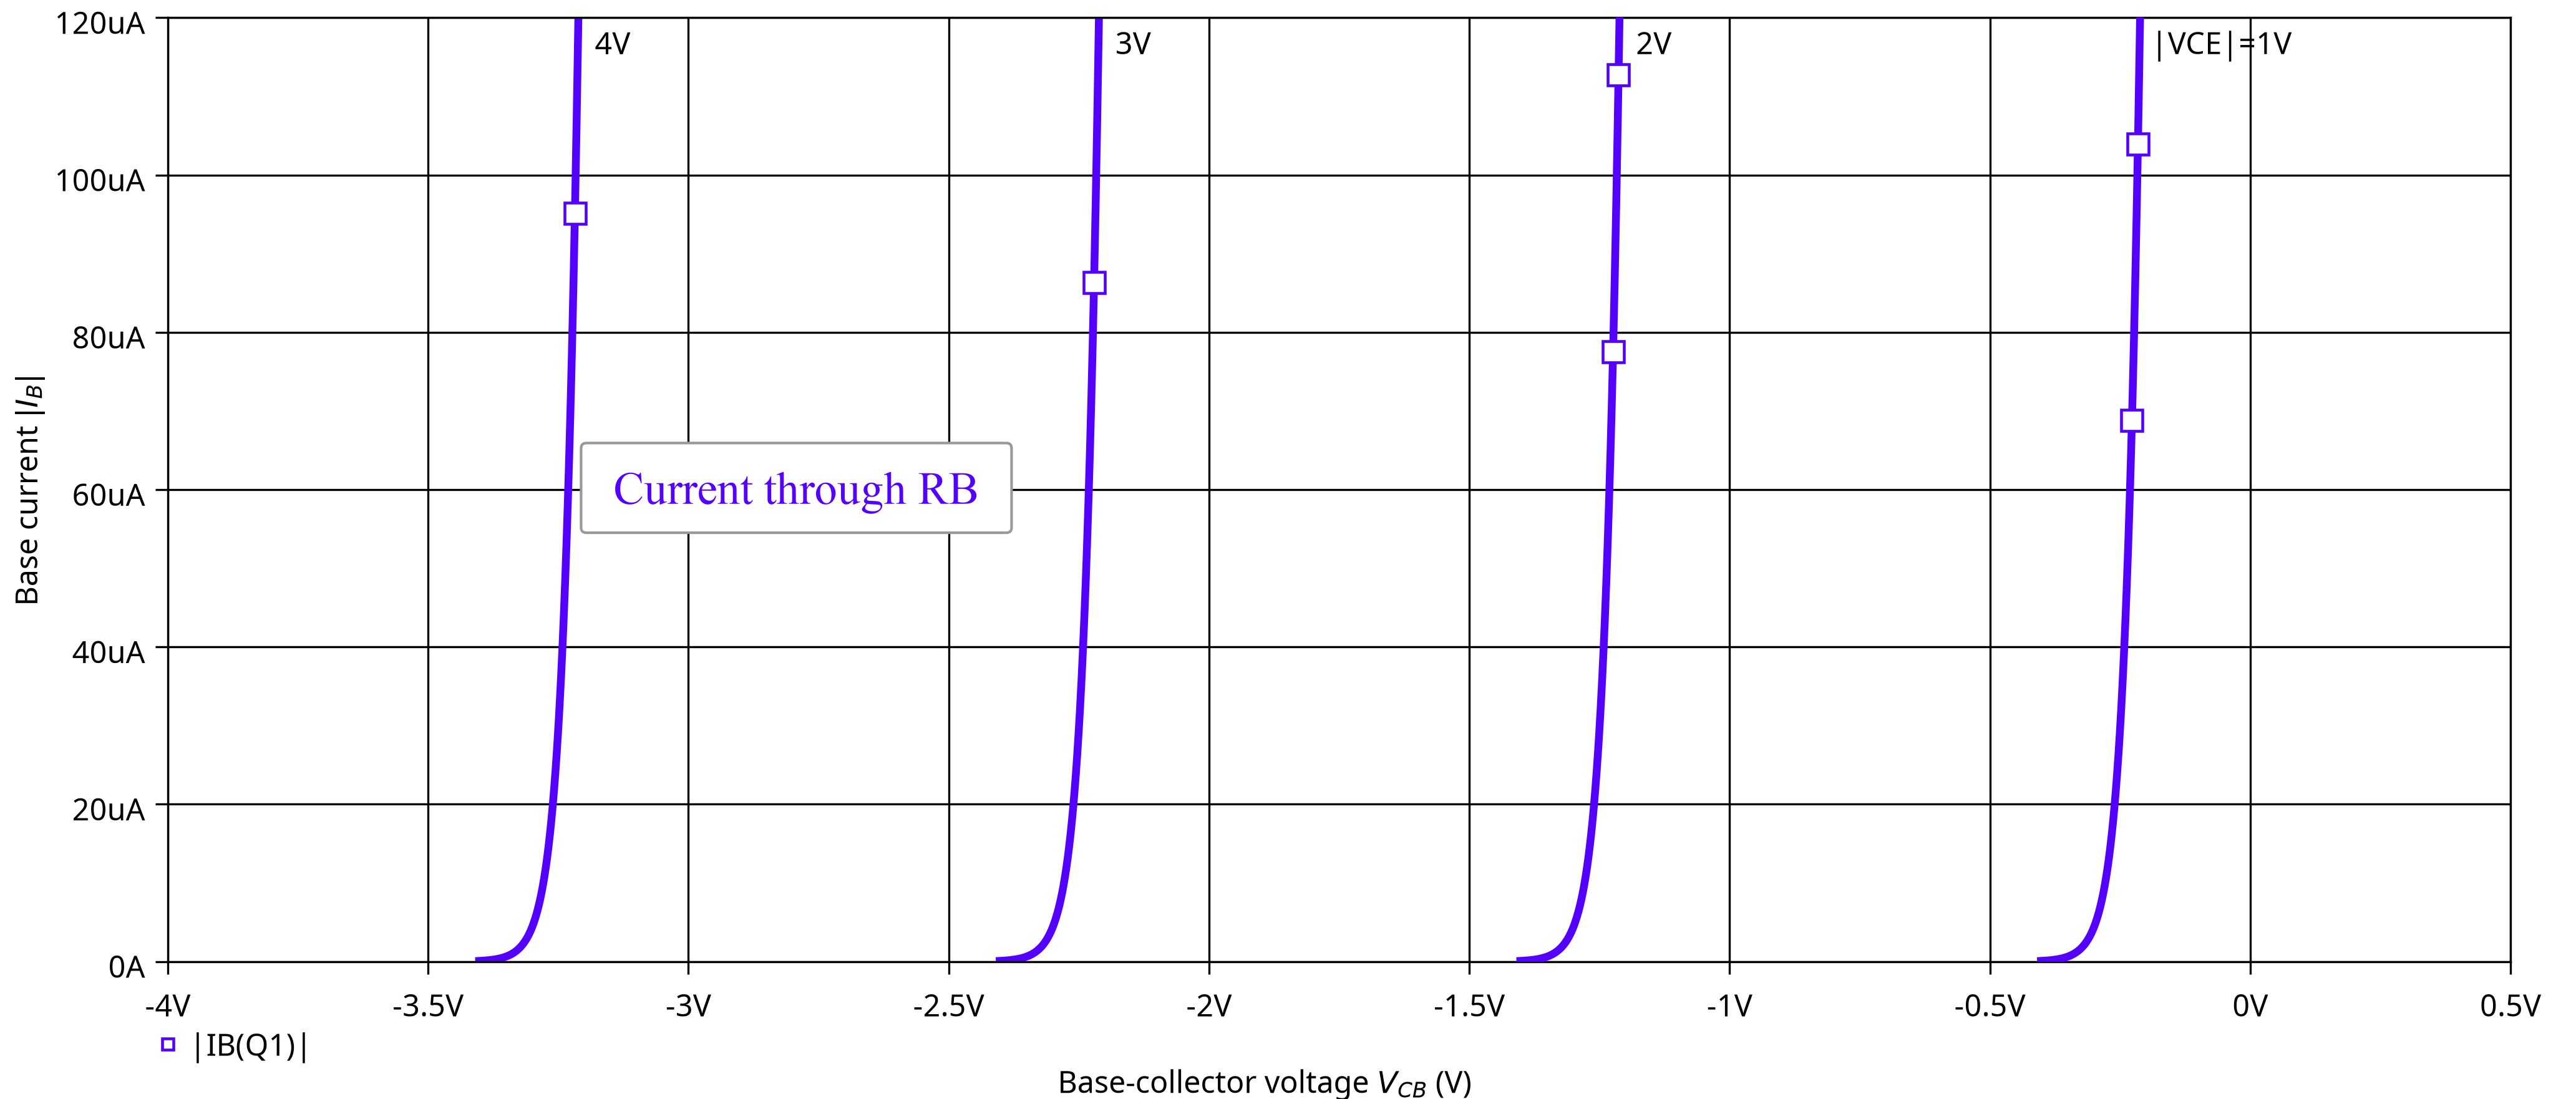
\includegraphics[width=\textwidth]{cc_input_pnp.png}
		\caption{PSpice output: input characteristic of the PNP transistor in CC configuration for $|V_{EE}| = 1$ to \SI{4}{\volt} ($|V_{CE}| = 1$ to \SI{4}{\volt}), plotted against $V_{BC}$; the four curves are separated by about \SI{1}{\volt}.}
		\label{fig:cc-in-pnp}
	\end{figure}
	
	\begin{figure}[H]
		\centering
		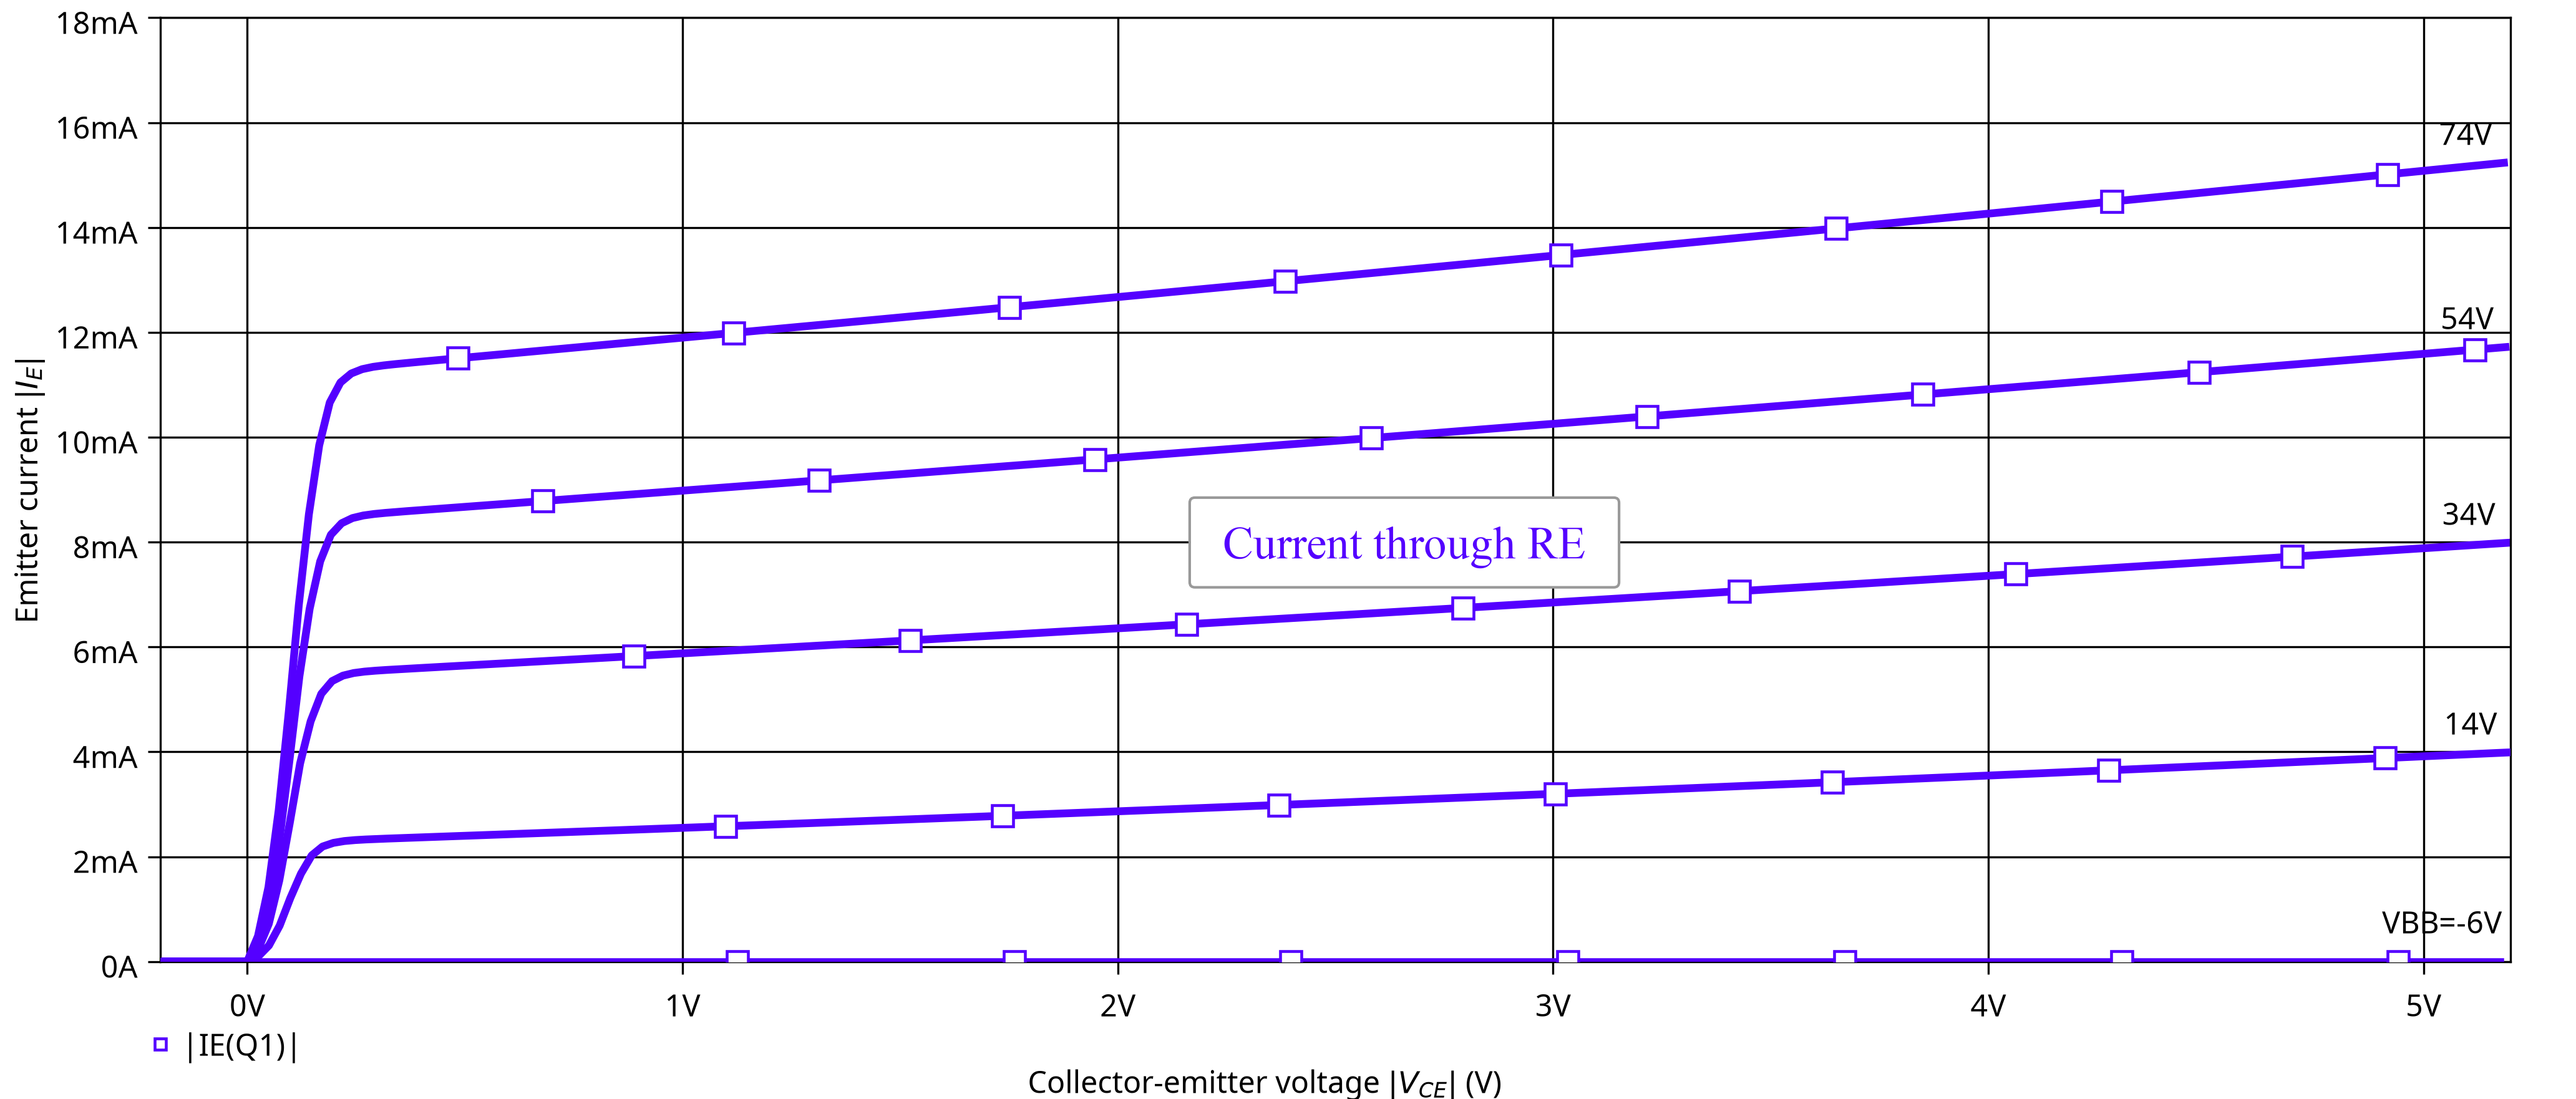
\includegraphics[width=\textwidth]{cc_output_pnp.png}
		\caption{PSpice output: output characteristic of the PNP transistor in CC configuration for $|V_{BB}| = -6$, 14, 34, 54 and \SI{74}{\volt} ($|I_B| \approx 0$ to \SI{74}{\micro\ampere}). The emitter current reaches \SI{11.59}{\milli\ampere} at $|V_{CE}| = \SI{5}{\volt}$ for the 54 V step.}
		\label{fig:cc-out-pnp}
	\end{figure}
	
	The PNP families in Figures~\ref{fig:cb-in-pnp} to~\ref{fig:cc-out-pnp}
	show the same features as the NPN families with the polarities reversed.
	The CB input curve reaches \SI{4.26}{\milli\ampere} at
	\SI{0.738}{\volt}, about \SI{35}{\milli\volt} higher than the NPN curve
	(\SI{4.30}{\milli\ampere} at \SI{0.703}{\volt}); this offset is set by the
	saturation current of the model, which is smaller for the 2N3906 than
	for the 2N3904. The \SI{45}{\volt} curve is shifted by about
	\SI{25}{\milli\volt}. The larger Early effect of the PNP model is clear
	in the output families: between \SI{5}{\volt} and \SI{10}{\volt} the CB
	current rises by \SI{8.5}{\micro\ampere} against \SI{3.1}{\micro\ampere}
	for the NPN, and the CE current at $I_B = \SI{52.36}{\micro\ampere}$
	rises by \SI{2.28}{\milli\ampere} over the same span. After the
	correction to constant input current these slopes give
	$R_{\mathrm{out,CB}} = \SI{1.445}{\mega\ohm}$,
	$R_{\mathrm{out,CE}} = \SI{2.190}{\kilo\ohm}$ and
	$R_{\mathrm{out,CC}} = \SI{2.075}{\kilo\ohm}$, about 2.4, 4.0 and 4.1
	times lower than the NPN values, so the lower Early voltage of the PNP
	model is reflected directly in the output slopes. The current gains are
	also closer to the reference value $\beta = 200$ for the PNP, with
	$\beta = 188.0$ and $\gamma = 185.5$.
	
	\subsection{Operating regions}
	The regions were identified from the output families as described in
	step 10 of the procedure. Table~\ref{tab:regions} lists the numerical
	boundaries. In cutoff both junctions are reverse biased, so the
	collector current for zero input current is only a leakage of about
	\SI{5}{\pico\ampere}, indistinguishable from the axis in the plots. The
	saturation knee is the lowest output voltage at which the trace has
	reached \SI{90}{\percent} of its value just inside the active region; to
	the left of it the collector junction is forward biased. The active
	region is everything to the right of the knee up to the end of the
	sweep, with the base-emitter junction forward biased above its turn-on
	voltage.
	
	\begin{table}[H]
		\centering
		\caption{Operating regions identified from the simulated families}
		\label{tab:regions}
		\renewcommand{\arraystretch}{1.25}
		\small
		\begin{tabular}{|l|c|c|}
			\hline
			\textbf{Boundary} & \textbf{NPN (2N3904)} & \textbf{PNP (2N3906)} \\
			\hline
			Cutoff: $I_C$ for $I_E = 0$, $|V_{CB}| = 5$ V (CB) & \SI{5.0}{\pico\ampere} & \SI{5.0}{\pico\ampere} \\
			\hline
			Cutoff: $I_C$ for $I_B = 0$, $|V_{CE}| = 5$ V (CE) & \SI{5.0}{\pico\ampere} & \SI{5.0}{\pico\ampere} \\
			\hline
			Saturation knee, CB ($I_E = 4$ mA) & $V_{CB} < \SI{-0.63}{\volt}$ & $V_{CB} > \SI{0.71}{\volt}$ \\
			\hline
			Saturation knee, CE (6 V step, $|I_B| \approx 52$ \si{\micro\ampere}) & $V_{CE} < \SI{0.21}{\volt}$ & $|V_{CE}| < \SI{0.19}{\volt}$ \\
			\hline
			Saturation knee, CC (54 V step, $|I_B| \approx 58$ \si{\micro\ampere}) & $V_{CE} < \SI{0.22}{\volt}$ & $|V_{CE}| < \SI{0.19}{\volt}$ \\
			\hline
			Active region (output families) & above the knee & above the knee \\
			\hline
			Turn-on: $V_{EB}$ at $I_E = 1$ mA (CB input) & \SI{0.664}{\volt} & \SI{0.700}{\volt} \\
			\hline
			Turn-on: $V_{BE}$ at $I_B = 10$ \si{\micro\ampere} (CE input) & \SI{0.674}{\volt} & \SI{0.721}{\volt} \\
			\hline
		\end{tabular}
	\end{table}
	
	\begin{table}[H]
		\centering
		\caption{Theoretical and simulated parameters of the NPN transistor
			(2N3904)}
		\label{tab:npn}
		\renewcommand{\arraystretch}{1.25}
		\begin{tabular}{|l|c|c|c|}
			\hline
			\textbf{Quantity} & \textbf{Theoretical} & \textbf{Simulated} & \textbf{\% Error} \\
			\hline
			$\alpha = \Delta I_C/\Delta I_E$ & 0.9950 & 0.9944 & $0.06$ \\
			\hline
			$\beta = \Delta I_C/\Delta I_B$ & 200.0 & 174.0 & $13.00$ \\
			\hline
			$\gamma = \Delta I_E/\Delta I_B$ & 201.0 & 173.8 & $13.53$ \\
			\hline
			$R_{\mathrm{in,CB}}$ & \SI{6.841}{\ohm} & \SI{7.242}{\ohm} & $-5.86$ \\
			\hline
			$R_{\mathrm{in,CE}}$ & \SI{614.7}{\ohm} & \SI{708.5}{\ohm} & $-15.26$ \\
			\hline
			$R_{\mathrm{in,CC}}$ & \SI{543.3}{\ohm} & \SI{645.4}{\ohm} & $-18.79$ \\
			\hline
			$R_{\mathrm{out,CB}}$ & \SI{4.213}{\mega\ohm} & \SI{3.497}{\mega\ohm} & $17.00$ \\
			\hline
			$R_{\mathrm{out,CE}}$ & \SI{8.880}{\kilo\ohm} & \SI{8.801}{\kilo\ohm} & $0.89$ \\
			\hline
			$R_{\mathrm{out,CC}}$ & \SI{8.174}{\kilo\ohm} & \SI{8.418}{\kilo\ohm} & $-2.99$ \\
			\hline
		\end{tabular}
	\end{table}
	
	\begin{table}[H]
		\centering
		\caption{Theoretical and simulated parameters of the PNP transistor
			(2N3906)}
		\label{tab:pnp}
		\renewcommand{\arraystretch}{1.25}
		\begin{tabular}{|l|c|c|c|}
			\hline
			\textbf{Quantity} & \textbf{Theoretical} & \textbf{Simulated} & \textbf{\% Error} \\
			\hline
			$\alpha = \Delta I_C/\Delta I_E$ & 0.9950 & 0.9953 & $-0.03$ \\
			\hline
			$\beta = \Delta I_C/\Delta I_B$ & 200.0 & 188.0 & $6.00$ \\
			\hline
			$\gamma = \Delta I_E/\Delta I_B$ & 201.0 & 185.5 & $7.71$ \\
			\hline
			$R_{\mathrm{in,CB}}$ & \SI{6.906}{\ohm} & \SI{7.201}{\ohm} & $-4.27$ \\
			\hline
			$R_{\mathrm{in,CE}}$ & \SI{620.9}{\ohm} & \SI{631.0}{\ohm} & $-1.63$ \\
			\hline
			$R_{\mathrm{in,CC}}$ & \SI{543.8}{\ohm} & \SI{575.3}{\ohm} & $-5.79$ \\
			\hline
			$R_{\mathrm{out,CB}}$ & \SI{1.719}{\mega\ohm} & \SI{1.445}{\mega\ohm} & $15.94$ \\
			\hline
			$R_{\mathrm{out,CE}}$ & \SI{2.256}{\kilo\ohm} & \SI{2.190}{\kilo\ohm} & $2.93$ \\
			\hline
			$R_{\mathrm{out,CC}}$ & \SI{2.091}{\kilo\ohm} & \SI{2.075}{\kilo\ohm} & $0.77$ \\
			\hline
		\end{tabular}
	\end{table}
	
	\begin{table}[H]
		\centering
		\caption{Comparison of the three configurations for both transistors}
		\label{tab:compare}
		\renewcommand{\arraystretch}{1.25}
		\begin{tabular}{|l|c|c|c|}
			\hline
			\textbf{Configuration} & \textbf{Current gain} & \textbf{Input resistance} & \textbf{Output resistance} \\
			\hline
			CB (NPN) & $\alpha = 0.9944$ & \SI{7.242}{\ohm} & \SI{3.497}{\mega\ohm} \\
			\hline
			CE (NPN) & $\beta = 174.0$ & \SI{708.5}{\ohm} & \SI{8.801}{\kilo\ohm} \\
			\hline
			CC (NPN) & $\gamma = 173.8$ & \SI{645.4}{\ohm} & \SI{8.418}{\kilo\ohm} \\
			\hline
			CB (PNP) & $\alpha = 0.9953$ & \SI{7.201}{\ohm} & \SI{1.445}{\mega\ohm} \\
			\hline
			CE (PNP) & $\beta = 188.0$ & \SI{631.0}{\ohm} & \SI{2.190}{\kilo\ohm} \\
			\hline
			CC (PNP) & $\gamma = 185.5$ & \SI{575.3}{\ohm} & \SI{2.075}{\kilo\ohm} \\
			\hline
		\end{tabular}
	\end{table}
	
	% =====================================================================
	\section{Discussion}
	% =====================================================================
	The simulated families reproduce the expected behavior of the three
	configurations. The CB connection gives a current gain just below unity,
	the smallest input resistance (\SI{7.242}{\ohm}) and the largest output
	resistance (\SI{3.497}{\mega\ohm}); the CE connection gives a large
	current gain and an input resistance about ninety-eight times larger
	(\SI{708.5}{\ohm}), with an output resistance about four hundred times
	smaller (\SI{8.801}{\kilo\ohm}); the CC connection repeats the CE input
	characteristic and delivers the emitter current as its output, with a
	current gain of \num{173.8} and an output resistance of
	\SI{8.418}{\kilo\ohm}, of the same order as the CE value.
	Table~\ref{tab:compare} shows these trends for both polarities, and they
	explain why a CB stage is used as a current buffer, a CC stage as a
	voltage buffer and a CE stage for gain. The measured $\gamma$ agrees with
	$\beta$ to within \SI{0.2}{\percent} but does not exceed it by one,
	because the two gains are read at different base currents and the
	differential gain of the model varies with the current. The cutoff,
	active and saturation regions of Table~\ref{tab:regions} agree with the
	junction-bias picture of Section~\ref{sec:theory}: the saturation knee
	lies where the collector junction becomes forward biased, at
	$V_{CB} \approx \SI{-0.6}{\volt}$ to \SI{-0.7}{\volt}, and therefore at
	$V_{CE} = V_{CB} + V_{BE}$ of only a fraction of a volt (\SIrange{0.19}{0.22}{\volt}
	is read from the CE and CC families).

	The percentage errors are smallest for the current gain $\alpha$ and for
	the CE and CC output resistances, which agree with theory to within
	\SI{3}{\percent} for both transistors, and largest for the NPN input
	resistances (\SI{15.26}{\percent} and \SI{18.79}{\percent}), the CB
	output resistance (\SI{17.00}{\percent} for the NPN and
	\SI{15.94}{\percent} for the PNP) and the NPN current gains
	(about \SI{13}{\percent}). The gain error is not a simulation defect: the
	theoretical $\beta = 200$ is the middle of the datasheet range
	$h_{FE} = 100$ to 300 at \SI{10}{\milli\ampere}, not a value that the
	datasheet specifies as typical, whereas the 2N3904 model card sets
	$I_{SE} = I_S$ with an ideality factor of 1.259, so its base current
	contains a large recombination component and its own gain at
	\SI{10}{\milli\ampere} is only about 170. The measured
	\SI{13.00}{\percent} deviation therefore compares the model with the
	datasheet mid-range value, not with itself; the same effect makes
	$\Delta V_{BE}$ larger than $V_T\ln(I_2/I_1)$, so the NPN input
	resistances are \SI{15.26}{\percent} and \SI{18.79}{\percent} above the
	ideal values. The PNP model has $I_{SE} = 0$, so its base current is
	nearly ideal and its input-resistance errors fall to
	\SI{1.63}{\percent} and \SI{5.79}{\percent}. The CB output resistance is
	the least reliable entry in both tables because its theoretical value is
	the difference of two almost equal values of $\alpha$, only
	$2.8\times10^{-4}$ apart for the NPN and $6.8\times10^{-4}$ for the PNP;
	a small change in the slope moves it by a large percentage, although the
	measured value is still of the order of megohms, as predicted.

	The Early voltage controls the output slope directly: the PNP model has
	$V_A = \SI{18.7}{\volt}$ against \SI{74.03}{\volt} for the NPN, and the
	measured PNP output resistances are lower by close to the corresponding
	ratio of 3.96 (\SI{2.19}{\kilo\ohm} against \SI{8.80}{\kilo\ohm} in CE,
	and \SI{2.08}{\kilo\ohm} against \SI{8.42}{\kilo\ohm} in CC). The CC
	input characteristic is plotted against $V_{BC}$ because that is the
	variable of the task-sheet resistance; at constant $V_{CE}$ it differs
	from $V_{BE}$ only by the constant $V_{CE}$, so the four curves are
	shifted sideways by \SI{1}{\volt} each. The main limitation is that all
	the resistances are chord slopes of DC characteristics, so they include
	the series base and collector resistances of the model; a small-signal AC
	analysis at the same operating point would give values closer to the
	ideal $r_e$, $r_\pi$ and $r_o$ formulas.

	\clearpage
	% =====================================================================
	\section{Reference}
	% =====================================================================
	\renewcommand{\refname}{} % suppress the duplicate "References" heading
	\sloppy
	\begin{thebibliography}{9}
		\bibitem{ref:sedra} A. S. Sedra and K. C. Smith,
		\textit{Microelectronic Circuits}, 7th ed. New York, NY, USA:
		Oxford University Press, 2015.
		\bibitem{ref:theraja} B. L. Theraja and A. K. Theraja,
		\textit{A Textbook of Electrical Technology}, vol.~IV:
		\textit{Electronic Devices and Circuits}, multicolour ed. New Delhi,
		India: S. Chand \& Company, 2006.
		\bibitem{ref:2n3904} ON Semiconductor, ``2N3904 NPN general-purpose
		amplifier,'' datasheet. [Online]. Available:
		https://www.farnell.com/datasheets/3770732.pdf. [Accessed:
		Nov.~21, 2026].
		\bibitem{ref:2n3906} Fairchild Semiconductor, ``2N3906 / MMBT3906 /
		PZT3906 PNP general-purpose amplifier,'' datasheet, Rev.~1.2.2,
		Apr.~2014. [Online]. Available:
		https://www.farnell.com/datasheets/2277422.pdf. [Accessed:
		Nov.~21, 2026].
	\end{thebibliography}
	
\end{document}
